\documentclass[12pt, openany]{report}
\usepackage[utf8]{inputenc}
\usepackage[T1]{fontenc}
\usepackage{amsmath,amsfonts,amssymb}
\usepackage{amssymb}
\usepackage{multicol}
\usepackage[a4paper,left=2.5cm,right=2.5cm,top=2.5cm,bottom=2.5cm]{geometry}
\usepackage[english]{babel}
\usepackage{libertine}
\usepackage{graphicx}
\usepackage{wrapfig}
\usepackage{amsthm}
\usepackage{float}
\usepackage{enumitem}
\usepackage{pythonhighlight}
\usepackage[]{titletoc}
\usepackage{empheq}
\usepackage{titlesec}
\usepackage{mathpazo}
\usepackage{xfrac}
\usepackage{textcomp}
\usepackage{mathtools}
\usepackage{caption}
\usepackage{tabularray}
\usepackage{subcaption}
\usepackage[bottom]{footmisc}
\usepackage{pdfpages}
\usepackage{tabularx}
\usepackage[skins]{tcolorbox}

\theoremstyle{definition}
\newtheorem{thm}{Theorem}[chapter]
\newtheorem{definition}[thm]{Definition}
\newtheorem{lem}[thm]{Lemma}
\newtheorem{crl}[thm]{Corollary}

\titleformat{\chapter}[display]
  {\normalfont\bfseries}{}{0pt}{\Huge}
\usepackage{hyperref}
\newcommand{\hsp}{\hspace{20pt}}
\newcommand{\HRule}{\rule{\linewidth}{0.5mm}}

\newcommand{\R}{\mathbb{R}}
\newcommand{\C}{\mathbb{C}}

\let\oldemptyset\emptyset
\let\emptyset\varnothing

\hbadness=10001
\hfuzz=200pt

\begin{document}
\begin{titlepage}
    \begin{sffamily}
    \begin{center}
        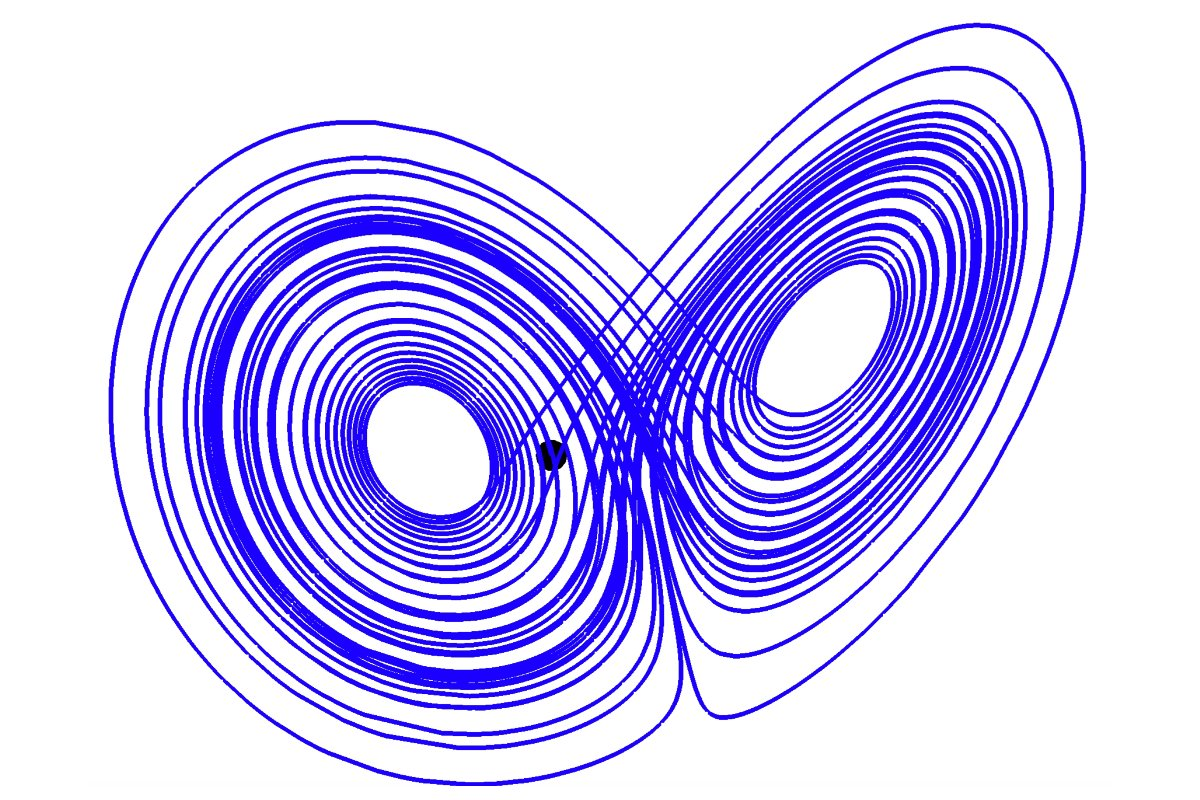
\includegraphics[scale=0.25]{img/page_de_garde.png} \\[1cm]
        \HRule \\[0.4cm]
        { \huge \bfseries LINMA2370 Modelling and Analysis of Dynamical Systems \\[0.4cm] }
    
        \HRule \\[1.5cm]
        \textsc{\LARGE Simon Desmidt}\\[1cm]
        \vfill
        \vspace{2cm}
        {\large Academic year 2024-2025 - Q1}
        \vspace{0.4cm}
         
        
\includegraphics[width=0.15\textwidth]{img/epl.png}
        
        UCLouvain\\
    
    \end{center}
    \end{sffamily}
\end{titlepage}

\setcounter{tocdepth}{1}
\tableofcontents
\chapter{Introduction}
The tools introduced in this course are a simplifying view of the reality, yet very uselful to build simple and effective models in view of the control and optimization of the dynamical behaviour of the real systems.
\section{Reminders}
\begin{itemize}
    \item A subset of \(\R\) is said to be negligible if its Lebesgue measure is equal to zero and that a property is said to be true almost everywhere if it is false only on a negligible set. 
    \item Let \(I\subseteq \R\) be an interval the interior of which is not empty. A function \(x:I\rightarrow \R^N\) is said to be absolutely continuous if 
\end{itemize}
\begin{multline*}
        \forall \varepsilon \in (0,\infty),\: \exists \delta\in (0,\infty) \: : \\
        \forall n\in \mathbb{N}\setminus\{0\},\: \forall a_1,b_1,\dots, a_n,b_n\in I : \\ 
        a_i<b_i \: \forall i\in \{1,\dots,n\}, \: b_i\le a_{i+1} \:\forall i\in \{1,\dots,n-1\}, \\
        \sum_{i=1}^n(b_i-a_i)\le \delta \Longrightarrow \sum_{i=1}^n \lVert x(b_i)-x(a_i)\rVert \le \varepsilon
\end{multline*}
\begin{itemize}
    \item Let \(a,b\in \R\) with \(a<b\). A function \(x:[a,b]\rightarrow \R\) is absolutely continuous iff there exists an integrable function \(\varphi:[a,b]\rightarrow \R\) such that, for every \(t\in [a,b]\), \[x(t) = x(a0) + \int_a^t \phi(s)ds\] in which case \(x\) is almost everywhere differentiable with \(\dot x(t) = \phi(t)\) for almost every \(t\in [a,b]\). 
    \item A function \(f:\Omega\rightarrow \R^N\), where \(\Omega\) is a nonempty subset of \(\R\times \R^N\), is said to be Lipschitz continuous in the second argument, uniformly with respect to the first argument, if there exists \(L\in \left[0,\infty\right)\) such that forall \(t\in \R\) and all \(x,y\in \R^N\) such that \((tx,),(t,y)\in \Omega\), \[\lVert f(t,x)-f(t,y)\rVert \le L\lVert x-y\rVert\] It is said to be locally Lipschitz continuous on an open ball for each argument. 
    \item Let \(\Omega\) be a nonempty open subset of \(\R\times \R^N\) and \(f:\Omega\rightarrow \R^N\) be such that 
    \begin{itemize}
        \item for all \(t\in \R,\: f(t,\cdot):\Omega_t\rightarrow \R^N\)
        \item \(\partial_2f:\Omega \rightarrow \mathcal{L}(\R^N,\R^N):(t,x)\rightarrow \partial_2f(t,x)\) is locally bounded.
    \end{itemize}
\end{itemize}
Then, \(f\) is locally Lipschitz continuous in the second argument, uniformly with respect to the first argument.
\begin{itemize}
    \item If \((X,\lVert \cdot \rVert_X)\) and \((Y,\lVert \cdot \rVert_Y)\) are two real normed spaces, and the real vector space \(\mathcal{L}(X,Y)\) of all continuous linear mappings from \(X\) to \(Y\)\footnote{Meaning matrix from \(X\) to \(Y\)} is equipped with the norm defined by \[\lVert L\rVert \coloneqq \sup_{x\in X\setminus\{0\}}\frac{\lVert Lx\rVert_Y}{\lVert x\rVert_X}\]
\end{itemize}
\section{State-space model}
A state-space model for a continuous dynamical system consists of an ODE of the form 
\begin{equation}\label{eq:1}
    \dot x (t) = f(t,x(t))
\end{equation}
where the function \(f:\Omega\rightarrow \R^N\), \(\Omega\) being a nonempty subset of \(\R\times \R^N\), is called the vector field associated with the ODE.
A continuous dynamical system with input \(u:\R\rightarrow \R^M\) described by the ODE 
\begin{equation}
    \dot x(t) = g(x(t),u(t))
\end{equation}
for some function \(g:\R^N\times \R^M\rightarrow \R^N\), can be written in the form \eqref{eq:1} by defining the vector field
\begin{equation}
    f_u :\R\times \R^N \rightarrow \R^N :(t,x) \rightarrow g(x,u(t))
\end{equation}
\begin{itemize}
    \item [\(\rightarrow\)] Note: the norm of each \((t,x)\in \R\times \R^N\)  is defined as \(|t|+\lVert x\rVert\).
\end{itemize}
\section{Integral curve}
Let \(\Omega\) be a nonempty subset of \(\R\times \R^N\). An integral curve of \(f:\Omega\rightarrow \R^N\) is a function \(x:I\rightarrow \R^N\) where \(I\subseteq \R\) is an interval, for which the interior is not empty, called the interval of existence of \(x\), i.e. differentiable and satisfies \((t,x(t))\in \Omega\) and \(\dot x(t) = f(t,x(t))\) for all \(t\in I\). The graph \(\{(t,x(t))|t\in I\}\) and the image \(\{x(t)|t\in I\}\) of \(x\) are respectively called the trajectory and the orbit of \(x\). Given an initial condition \((t_0,x_0)\in \Omega\), a solution to the initial value problem 
\begin{equation}
    \begin{cases}
        \dot x(t) = f(t,x(t))\\
        x(t_0) = x_0\\
    \end{cases}
\end{equation}
is an integral curve \(x:I\rightarrow \R^N\) of \(f\) such that \(t_0\in I\) and \(x(t_0)=x_0\). \\

If, for the IVP described hereabove, \(f\) is continuous, then a continuous function \(x:I\rightarrow \R^N\) where \(I\subseteq \R\) is an interval containing \(t_0\) and the interior of which is not empty, is a solution iff its graph is contained in \(\Omega\) and it satisfies the integral equation \[x(t)=x_0+\int_{t_0}^tf(s,x(s))ds\] for all \(t\in I\). In that case, \(\dot x\) is continuous. \\

Let \(\Omega\) be a nonempty subset of \(\R\times \R^N\). An integral curve in the extended sense of \(f:\Omega\rightarrow \R^N\) is a function \(x:I\rightarrow \R^N\), where \(I\subseteq \R\) is an interval the interior of which is not empty called the interval of existence of \(x\), that is absolutely continuous and satisfies \((t,x(t))\in \Omega\) for every \(t\in I\) and \(\dot x(t) = f(t(x(t)))\) for almost every \(t\in I\). 
\begin{itemize}
    \item [\(\rightarrow\)] Note: If \(f\) is continuous, then the two definitions of integral curves are equivalent.
\end{itemize}
\section{Existence of a solution}
Consider the IVP defined hereabove with an integral curve in the extended sense, under the following assumptions:
\begin{itemize}
    \item there exists \(\tau,r\in (0,\infty)\), such that \([t_0-\tau,t_0+\tau]\times B(x_0,r)\subseteq \Omega\);
    \item for every \(x\in B(x_0,r)\), the function \([t_0-\tau,t_0+\tau]\rightarrow \R^N:t\rightarrow f(t,x)\) is measurable;
    \item for every \(t\in [t_0-\tau,t_0+\tau]\), the function \(B(x_0,r)\rightarrow \R^N:x\rightarrow f(t,x)\) is continuous;
    \item there exists an integrable function \(m:[t_0-\tau,t_0+\tau]\rightarrow \left[0,\infty\right)\) such that \[\lVert f(t,x)\rVert \le m(t) \text{ for all }(t,x) \in [t_0-\tau,t_0\tau]\times B[x_0,r]\]
\end{itemize}
Then, there exists a solution defined on a compact interval the interior of which contains \(t_0\). \\
In particular, for the IVP with an integral curve in the general sense, if \((t_0,x_0)\) is an interior point of \(\Omega\) and \(f\) is continuous, then there exists a solution defined on a compact interval the interior of which contains \(t_0\).
\chapter{Dynamical systems and state-space models}
We will study first-order dynamical systems of the form 
\begin{equation}\label{eq:ODE}
    \dot x = f(x,u)
\end{equation}
where \(f\) is a mapping from \(\R^{n+m}\) to \(\R^n\), while \(x\) and \(u\) are vector functions of time, respectively the state and the input. 
\section{Terminology and notation}
\begin{itemize}
    \item We assume that the input is a piecewise continuous and bounded function: \(u\in \mathcal{U}\), where \(\mathcal{U}\) is a set of piecewise continuous and bounded functions from \(\R\) to \(\R^m\).
    \item For a given value of the initial state \(x(t_0)=x_0\) a,d a given input \(u\), the solution \(t\rightarrow x(t)\) for \(t\ge t_0\), of the system of ODE \ref{eq:ODE} is called the trajectory of the system. It is denoted \(x(t_0,x_0,u)\).
    \item When the input \(u\) can be freely chosen in \(\mathcal{U}\), the system \(\dot x = f(x,u)\) is said to be a forced/controlled system. 
    \item [\(\rightarrow\)] Note: in this course, we will study the solution of the equation \ref{eq:ODE} when the input is actually an a priori set constant: \(u(t) = \overline{u}\) \(\forall t\ge t_0\). The state-space model is then written as \(\dot x = f(x,\overline{u}) = f_{\overline{u}}(x)\).
\end{itemize}
\subsection{System with affine input}
\begin{equation}
    \dot x = f(x) + \sum_{i=1}^m u_ig_i = f(x) + G(x)u
\end{equation}
where \(f\) and \(g_i\) are mappings from \(\R^n\) to \(\R^n\). 
\subsection{System with affine state}
\begin{equation}
    \dot x = \sum_{i=1}^n x_ia_i(u) + b(u) = A(u)x+b(u)
\end{equation}
where \(b\) and \(a_i\) are mappings from \(\R^m\) to \(\R^n\). 
\subsection{Bilinear systems}
A bilinear system is affine both in the state and in the input:
\begin{equation}
    \dot x = \left(A_0 + \sum_{i=1}^mu_iA_i\right) x + B_0u 
\end{equation}
where \(A_i\) and \(B_i\) are matrices of dimensions \(n\times n\) and \(n\times m\) respectively. 
\subsection{Linear system}
\begin{equation}
    \dot x = Ax + Bu
\end{equation}
where \(A\) and \(B\) are matrices of dimensions \(n\times n\) and \(n\times m\) respectively. 
\chapter{State transformations}
\section{Definition}
The block diagram of a dynamical system is a visual representation of that system, necessarily containing \(n\) integrators whose outputs are the \(n\) state variables. \\
\begin{minipage}{.5\textwidth}
    \begin{figure}[H]
        \centering
        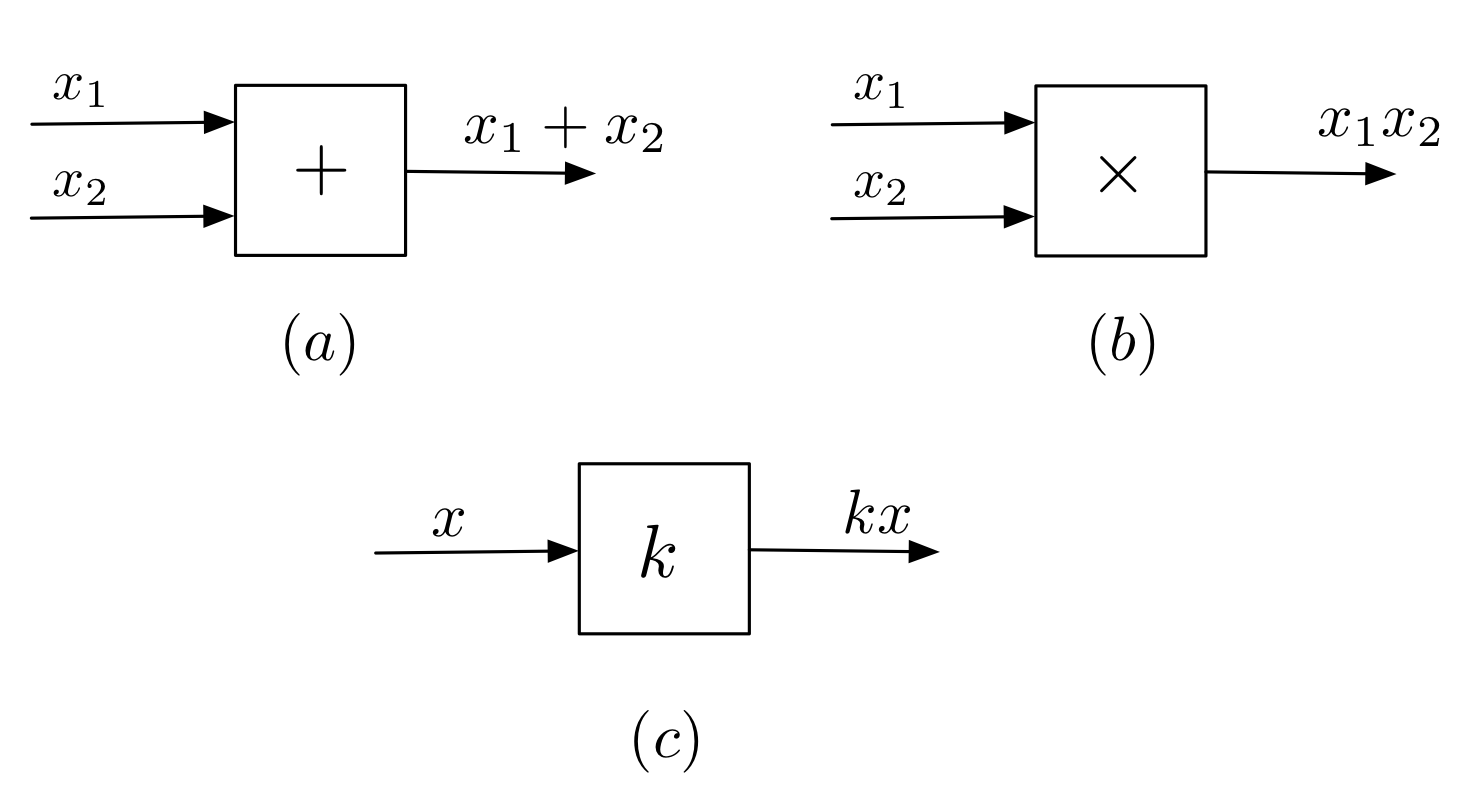
\includegraphics[width = \textwidth]{img/block_1.png}
    \end{figure}
\end{minipage}
\begin{minipage}{.5\textwidth}
    \begin{figure}[H]
        \centering
        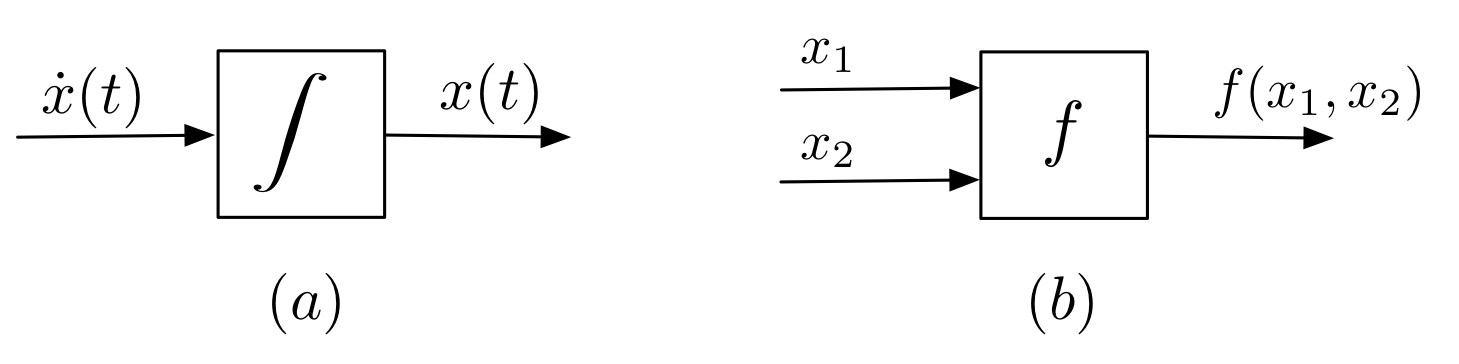
\includegraphics[width = \textwidth]{img/block_2.png}
    \end{figure}
\end{minipage}
The graph of a dynamical system contains as nodes the inputs and states of the system, and its edges are the relations between those quantities. The construction rules of the graph of a dynamical system are the following:
\begin{itemize}
    \item The \(n+m\) nodes are the \(n\) state variables \(x_i\) and the \(m\) inputs \(u_j\);
    \item there is an oriented edge from \(x_i\) (or \(u_k\)) to \(x_j\) if the varibale \(x_i\) (or \(u_k\)) appears explicitly in the equation of the derivative \(\dot x_j\).
\end{itemize}
Example for a DC electric machine: the state space model is 
\begin{equation}
    \begin{cases}
        \dot x_1 = x_2\\
        \dot x_2 = J^{-1}(-h(x_2)+K_mx_3x_4+u_3)\\
        \dot x_3 = L_s^{-1}(-R_sx_3+u_1)\\
        \dot x_4 = L_r^{-1}(-R_rx_4-K_ex_2x_3+u_2)\\
    \end{cases}
\end{equation}
and its graph representation is 
\begin{figure}[H]
    \centering
    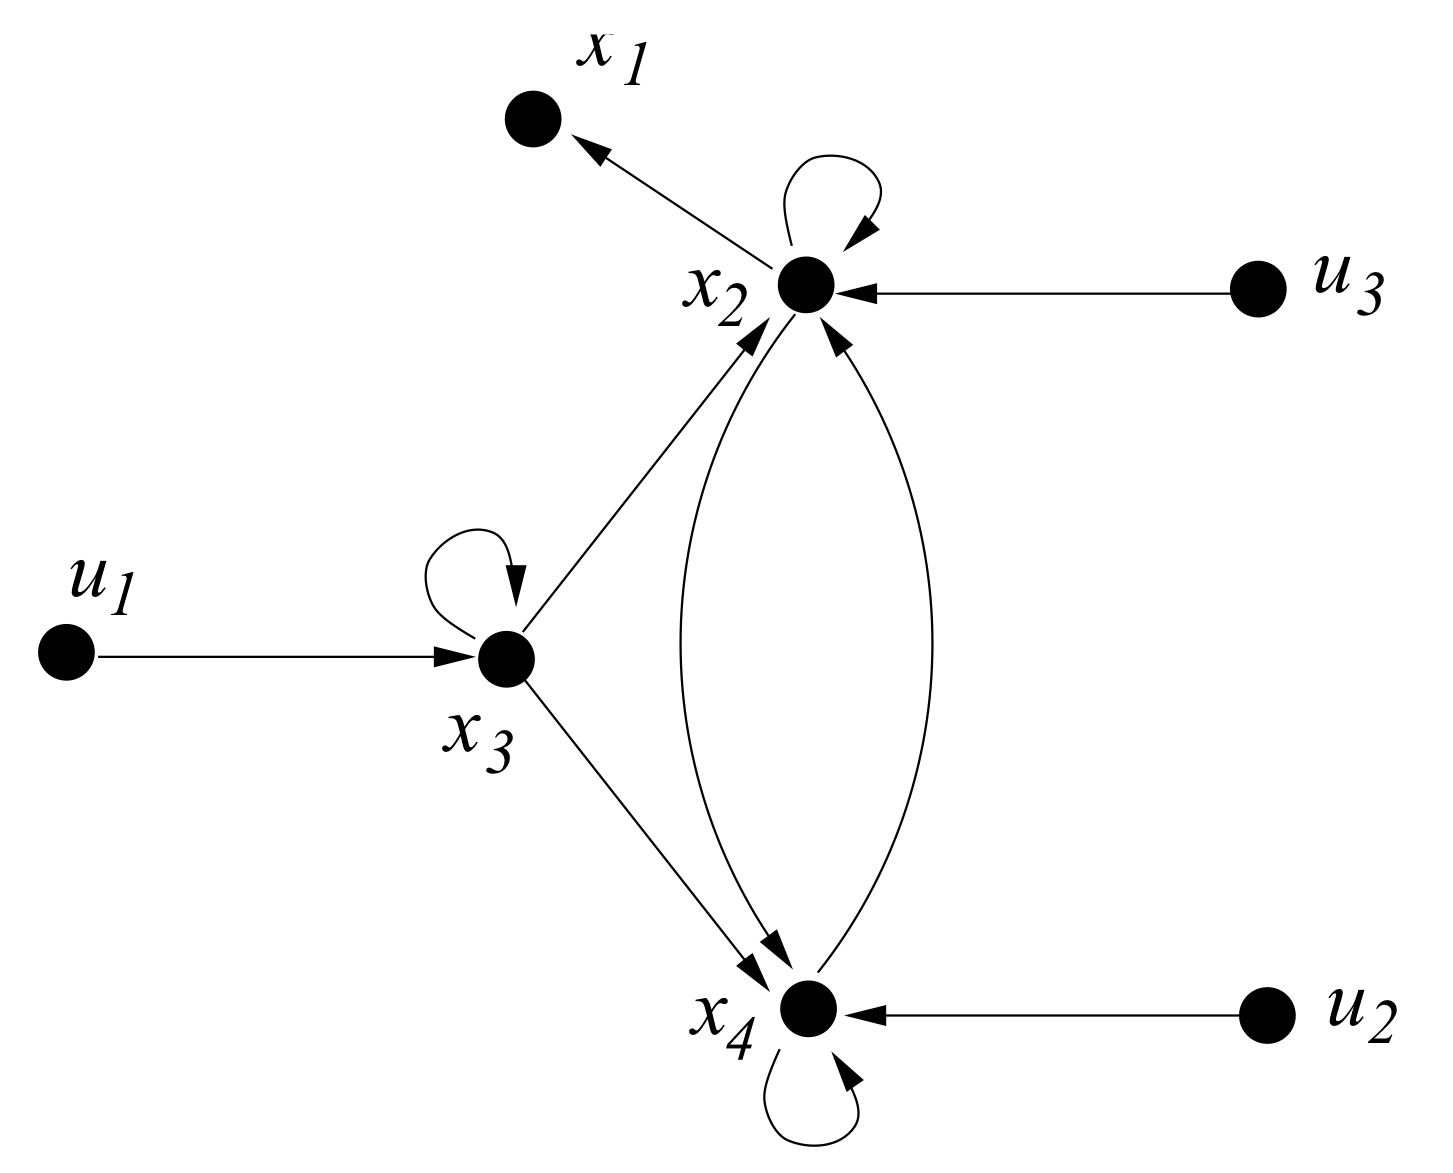
\includegraphics[width = .5\textwidth]{img/graph.png}
\end{figure}
\section{Linear state transformation}
For a dynamical system \(\dot x=f(x,u)\), a linear state transformation is a linear mapping \(T:\R^n\rightarrow \R^n\) that is bijective and transforms the state of the system \(x\in \R^n\) into a new state \(z\in \R^n\) following the rule \(z=Tx\), where \(T\in \R^{n\times n}\) is an invertible matrix. \\
The relation between the two systems is
\begin{equation}
    \begin{cases}
        \dot x=f(x,u)\\
        \dot z = g(z,u)\\
    \end{cases} \Longrightarrow \begin{cases}
        z\triangleq T^{-1}x\\
        g(z,u) \triangleq Tf(T^{-1}z,u)\\
    \end{cases}
\end{equation}
For a linear system, we have 
\begin{equation}
    \dot z = Fz+Gu \qquad F\triangleq TAT^{-1} \qquad G\triangleq TB
\end{equation}
\section{Nonlinear state transformation}
Let \(U,V\) be two open subsets of \(\R^n\). A nonlinear state transformation is a mapping \(T: U\rightarrow V\) that transforms the state of the system \(x\in U\) into a new state \(z\in V\): \(z=T(x)\) and that has the following properties:
\begin{itemize}
    \item \(T\) is bijective and has an inverse function \(T^{-1}:V\rightarrow U\) such that \(x=T^{-1}(z)\);
    \item \(T\) and \(T^{-1}\) are of class \(\mathcal{C}^1\), i.e. continuously differentiable. 
    \item [\(\rightarrow\)] Note: The state transformation is said to be global if \(U=V=\R^n\).
\end{itemize}
Such a transformation \(T\) is called a diffeomorphism, and the new state space is 
\begin{equation}
    \dot z = \frac{\partial T}{\partial x}\dot x = \frac{\partial T}{\partial x}f(x,u) \Longleftrightarrow f(x,u) \triangleq \left[\frac{\partial T^{-1}}{\partial z}g(z,u)\right]_{z=T(x)}
\end{equation}
\begin{lem}
    \begin{itemize}
        \item If the jacobien matrix \(\partial T/\partial x\) is nonsingular at \(x_0\), then, by the inverse function theorem, there is a neighbourhood \(U\) of \(x_0\) such that the mapping \(T\) restricted to \(U\) is a diffeomorphism on \(U\).
        \item \(T\) is a global diffeomorphism iff \begin{enumerate}
            \item \(\frac{\partial T}{\partial x}\) is a nonsingular for every \(x\in \R^n\);
            \item \(\lim_{\lVert x\rVert \rightarrow \infty} \lVert T(x)\rVert =\infty\).
        \end{enumerate}
    \end{itemize}
\end{lem}
\section{Triangular system}
\begin{definition}
    A single input dynamical system is triangular if there is a state variable \(x_i\) such that the shortest path from \(u\) t \(x_i\) in the graph of the system is of length \(n\).
\end{definition}
We can thus renumber the state variables such that the system is expressed as
\begin{align}\label{eq:triangular}
    \dot x_1 &= g_1(x_1,x_2) \nonumber\\
    &\vdots\nonumber\\
    \dot x_i &= g_i(x_1,\dots, x_{i+1})\nonumber\\
    & \vdots\nonumber\\
    \dot x_{n-1} &= g_{n-1}(x_1,\dots, x_n)\nonumber\\
    \dot x_n &= g_n(x_1,\dots,x_n,u)\tag{\theequation}  \refstepcounter{equation}
\end{align}
\section{Brunovsky canonical form}
\begin{definition} A single input dynamical system can be written in Brunovsky canonical form if there exists a state transformation \(T:U\rightarrow V\) and an open interval \(W\subseteq \R\) such that, in the new state variables \(z=T(x)\), the system takes on the following particular triangular form:
\begin{align}
    \dot z_1 &= z_2\nonumber\\
    \dot z_2 &= z_3\nonumber\\
    \vdots&\nonumber\\
    \dot z_n &= \alpha(z_1,\dots,z_n,u)\tag{\theequation}  \refstepcounter{equation}
\end{align}
where the function \(\alpha\) is continuous and invertible according to \(u\) over \(W\) for all \(z\in V\). The block diagram of the Brunovsky canonical form is
\begin{figure}[H]
    \centering
    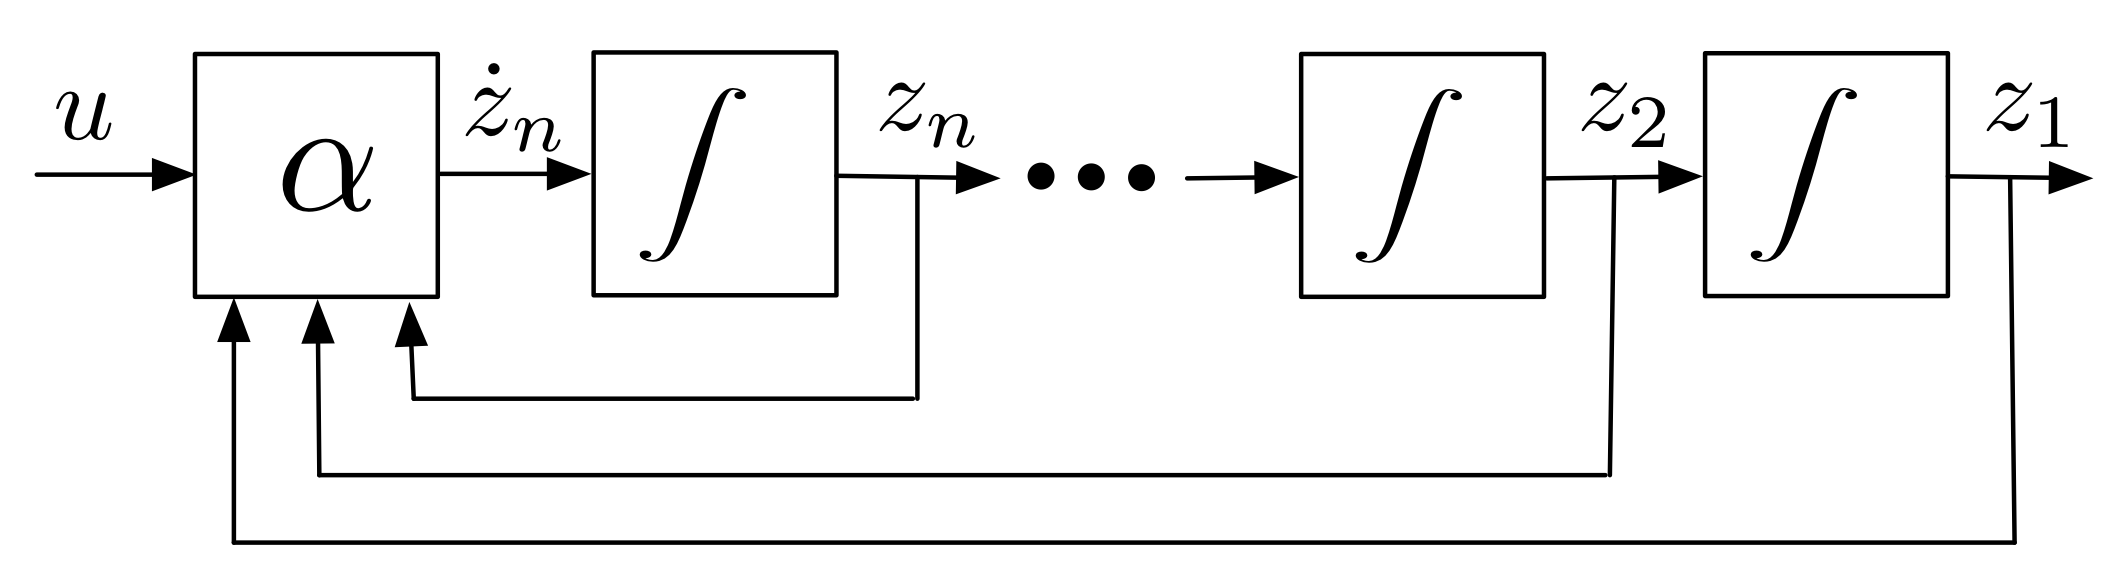
\includegraphics[width = .5\textwidth]{img/block_brunovsky.png}
\end{figure}
\end{definition}
\begin{lem}
    A triangular dynamical system described by the state-space model \eqref{eq:triangular} can be put under Brunovsky canonical form around \((x_0,u_0)\) if the inequalities 
    \begin{equation}
        \begin{cases}
            \frac{\partial g_i}{\partial x_{i+1}}\neq 0 \qquad i=1,\dots,n-1\\
            \frac{\partial g_n}{\partial u}\neq 0
        \end{cases}
    \end{equation}
\end{lem}
\begin{lem}
    A control-affine system \(\dot x =f(x)+g(x)u\) with \(x\in \R^n,u\in \R\) can be written in Brunovsky form in a domain \(U\subseteq \R^n\) if there exists a state transformation \(z=T(x)\) that fulfills the following conditions:
\end{lem}
\begin{itemize}
    \item \(T_{i+1}(x) = \frac{\partial T_i}{\partial x}f(x)\), for \(i=1,\dots,n-1\);
    \item \(\frac{\partial T_i}{\partial x}g(x)= 0\), for \(i=1,\dots,n-1\);
    \item \(\frac{\partial T_n}{\partial x}g(x)\neq 0\)
\end{itemize}
for every \(x\in U\).
\chapter{Equilibria and invariant sets}
In this chapter, we assume that \(f\) is locally Lipschitz continuous on an open set \(\Omega \subseteq \R^n\). 
\begin{definition}
    The pair \((\bar x, \bar u)\in \R^n\times \R^m\) is called an equilibrium of the system \(\dot x=f(x,u)\) if \(f(\bar x, \bar u)=0\). 
\end{definition}
\begin{definition}
    The equilibrium \((\bar x,\bar u)\) is said to be isolated if there exists a neighbourhood of \(\bar x\) that contains no other vector \(x\) such that \(f(x,\bar u)=0\).
\end{definition}
\section{Equilibria of linear systems}
\begin{equation}\label{eq:linear_sys}
    \dot x = Ax+Bu
\end{equation}
\begin{thm}
    If the matrix \(A\) is regular, then for each \(\bar u\), the pair \((-A^{-1}B\bar u, \bar u)\) is an isolated equilibrium.\\
    If the matrix \(A\) is singular, the system \eqref{eq:linear_sys} has a continuum of non-isolated equilibria provided that \(B\bar u\in Im(A)\). Those equilibria are the solutions of the system \(A\bar x=-B\bar u\), forming an affine space. On the other side, for each \(\bar u\) such that \(B\bar u\notin Im(A)\), the system does not have any equilibrium.
\end{thm}
\section{Invariant sets}
\begin{definition}
    A set \(\mathcal{X} \times U\subseteq \R^n\times \R^m\) is said to be (positively) invariant for the dynamical system \(\dot x=f(x,u)\) if, for all \(x_0\in \mathcal{X}\) and for all input signal \(t\rightarrow u(t)\in U\), the trajectory \(t\rightarrow x(t,x_0,u(t))\) remains in \(\mathcal{X}\) for all \(t\ge t_0\) whenever it is defined.
\end{definition}
\begin{definition}
    An outward normal vector to \(\mathcal{X}\subseteq \R^n\) at \(x\in \partial \mathcal{X}\) is a vector \(n\in \R^n\) such that \(n=\lambda(y-x)\), where \(\lambda >0\) and \(y\) is the center of an open ball \(B\subseteq \R^n\) such that \(x\in \partial B\) and \(B\cap \mathcal{X}=\emptyset\); if no such open ball exists, \(\mathcal{X}\) has no outward normal vector at \(x\). 
\end{definition}
\begin{thm}[Bony's theorem]
    Let \(f\) be a locally Lipschitz continuous vector field defined on an open set \(\Omega \subseteq \R^n\), and \(\mathcal{X}\) a closed set of \(\Omega\). If \(\langle f(x),n(x)\rangle \le 0\) for every \(x\in \partial \mathcal{X}\), and every vector \(n(x)\) is outward normal to \(\mathcal{X}\) at \(x\), then \(\mathcal{X}\) is (positively) invariant for \(f\).
\end{thm}
\begin{itemize}
    \item [\(\rightarrow\)] Note: no condition has to be verified at a point where \(\mathcal{X}\) does not have an outward normal vector.
\end{itemize}
\section{Periodic orbits}
A periodic orbit is such that it is arising from a trajectory of the dynamical system, verifying \(x(t)=x(t+T)\) for all \(t\) and for some \(T>0\)\footnote{Equilibria are trivial periodic orbits.}. The infimum of possible values for \(T\) is called the period of the trajectory.\\
We denote \(x(t,x_0,\bar u)\) as the solution at time \(t\) with \(x(t_0)=x_0\) and a constant input \(u(t) = \bar u\).
\begin{figure}[H]
    \centering
    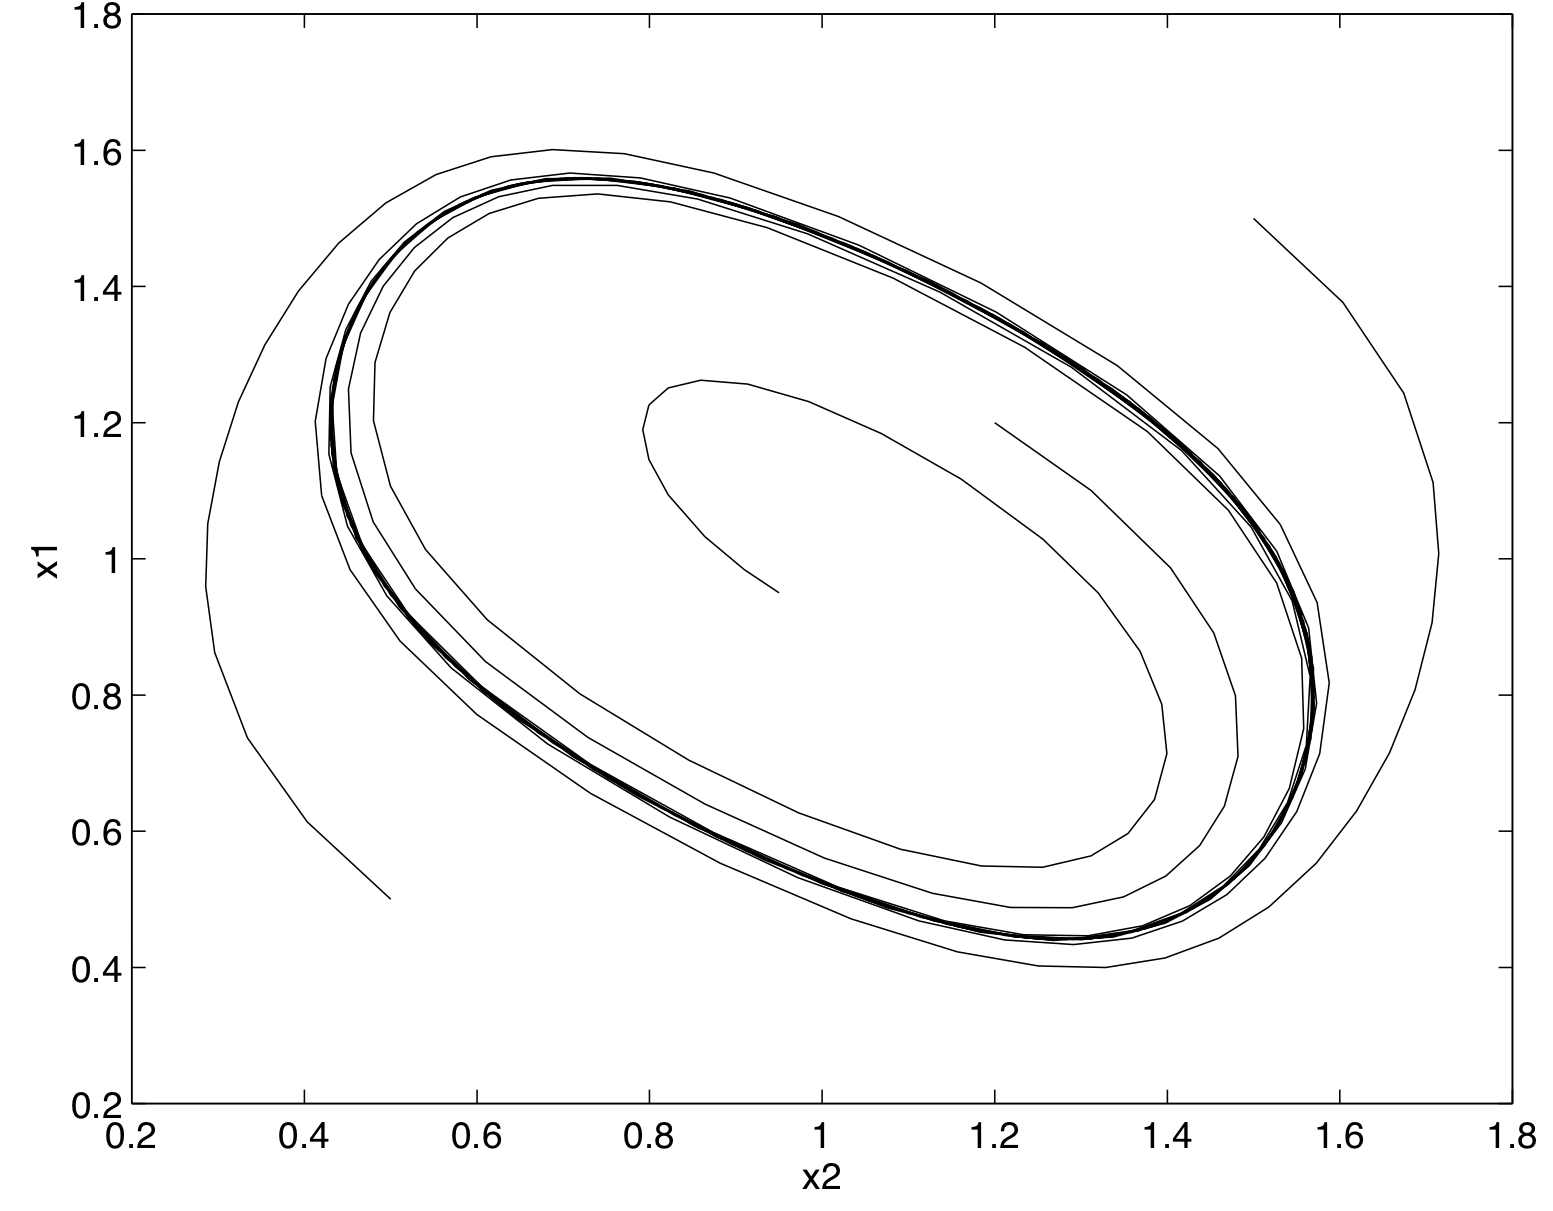
\includegraphics[width = .5\textwidth]{img/limit_cycle.png}
\end{figure}
\begin{definition}
    The point \(z\) is called a limit point of \(y\) for the dynamical system subject to a constant input \(\bar u\) if there exists a real sequence \(\{t_n\}_n\) such that \(t_n\rightarrow\infty\) when \(n\rightarrow \infty\) and \(\lim_{n\rightarrow\infty}x(t_n,y,\bar u)=z\).
\end{definition}
\begin{definition}
    A limit cycle is a closed orbit \(\gamma\) such that at least one point of \(\gamma\)\footnote{Implying that they all are.} is a limit point of at least another point of the phase plane not in \(\gamma\).
\end{definition}
\begin{itemize}
    \item [\(\rightarrow\)] Note: These definitions are only valid in \(\R^2\).
\end{itemize}
\begin{thm}[Bendixson-Dulac]
    Let \(D\) be a simply connected domain in \(\R^2\). If the divergence of \(f\)\footnote{\(\text{div}(f) = \frac{\partial f_1}{\partial x_1}+\frac{\partial f_2}{\partial x_2}\)} is not identically zero and does not change sign in \(D\), then \(D\) does not contain any closed orbit. 
\end{thm}
\begin{thm}[Poincar\'e-Bendixson]
    If \(E\) is a closed and bounded subset of \(\R^2\), invariant for the system \(\dot x=f(x,u)\), and if \(\gamma\) is an orbit starting in \(E\), then:
    \begin{itemize}
        \item either \(\gamma\) converges to an equilibrium (which is the unique limit point of \(\gamma\));
        \item or \(\gamma\) converges to a periodic orbit (which is the set of all limit points of \(\gamma\)).
    \end{itemize}
\end{thm}
This theorem can be used to prove the existence of a limit cycle:
\begin{enumerate}
    \item Find a compact invariant set (proved by showing that on the border of this set, the vector field points inwards);
    \item If there is no equilibrium in this set, it must contain a limit cycle or only periodic trajectories.
\end{enumerate}
\chapter{Local analysis of autonomous dynamical systems}
A dynamical system is said to be autonomous if the input is constant:
\begin{equation}
    \dot x= f(x,\bar u)
\end{equation}
\section{Linear planar systems}
Let us consider the linear planar system such as \eqref{eq:linear_sys} with constant input \(u=\bar u\). Let \(\bar x\) be an equilibrium point corresponding to \(\bar u\). We will use the state transformation \(z=M^{-1}(x-\bar x)\). We obtain the linear system
\begin{equation}
    \dot z = A'z\qquad A' = M^{-1}AM
\end{equation}
As \(A\) and \(A'\) have the same eigenvalues, we can choose \(A'\) to have a canonical form:
\begin{itemize}
    \item Two distinct real eigenvalues or double real eigenvalue (\(\lambda_1=\lambda_2\)) with a geometric multiplicity equal to 2.
\end{itemize}
\begin{equation}
    A' = \begin{bmatrix}
        \lambda_1 & 0\\
        0 & \lambda_2\\
    \end{bmatrix}
\end{equation}
\begin{itemize}
    \item Double real eigenvalue of geometric multiplicity equal to 1.
\end{itemize}
\begin{equation}
    A' = \begin{bmatrix}
        \lambda & 1\\
        0 & \lambda\\
    \end{bmatrix}
\end{equation}
\begin{itemize}
    \item Two complex conjugate eigenvalues \(\alpha \pm \omega i\).
\end{itemize}
\begin{equation}
    A' = \begin{bmatrix}
        \alpha & \omega\\
        -\omega & \alpha\\
    \end{bmatrix} \qquad \omega >0
\end{equation}
And the types of equilibrium for a linear planar system are:
\begin{figure}[H]
    \centering
    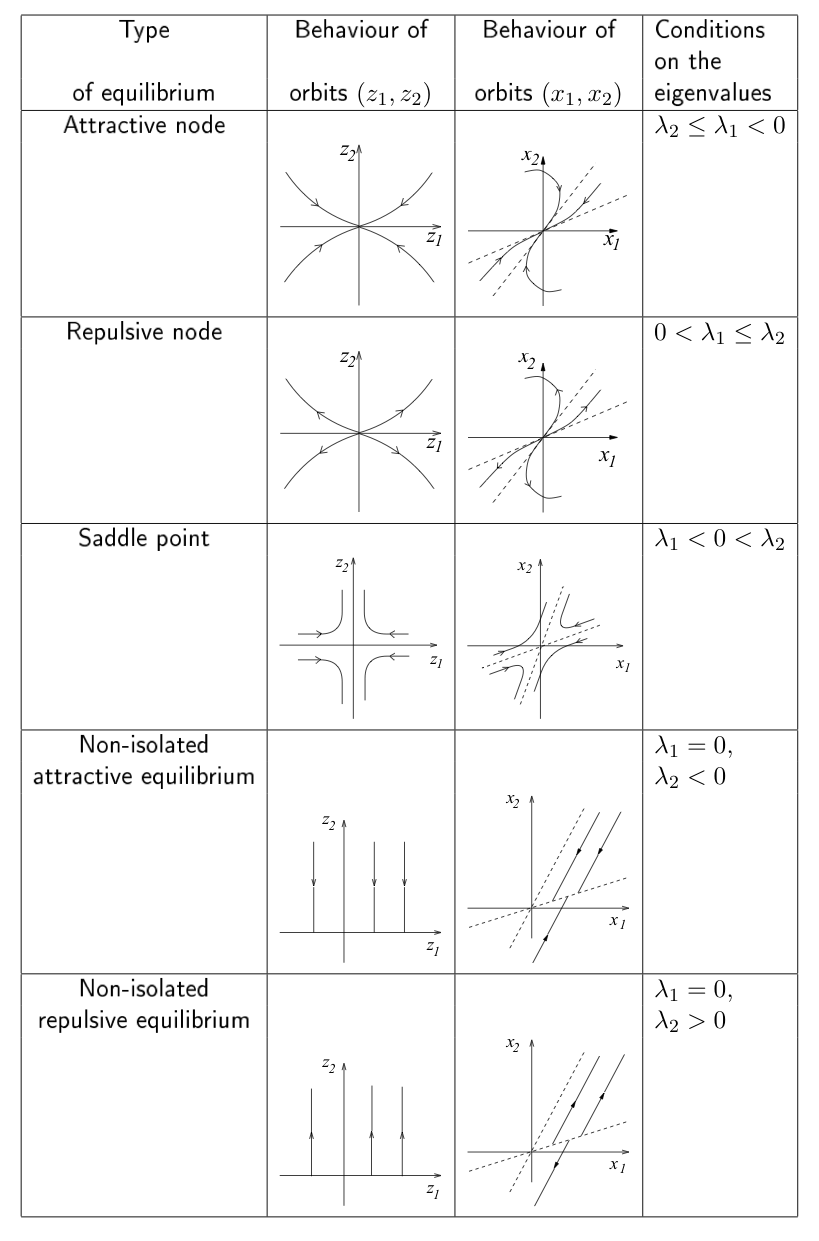
\includegraphics[width = \textwidth]{img/orbit_lin_sys_1.png}
\end{figure}
\begin{figure}[H]
    \centering
    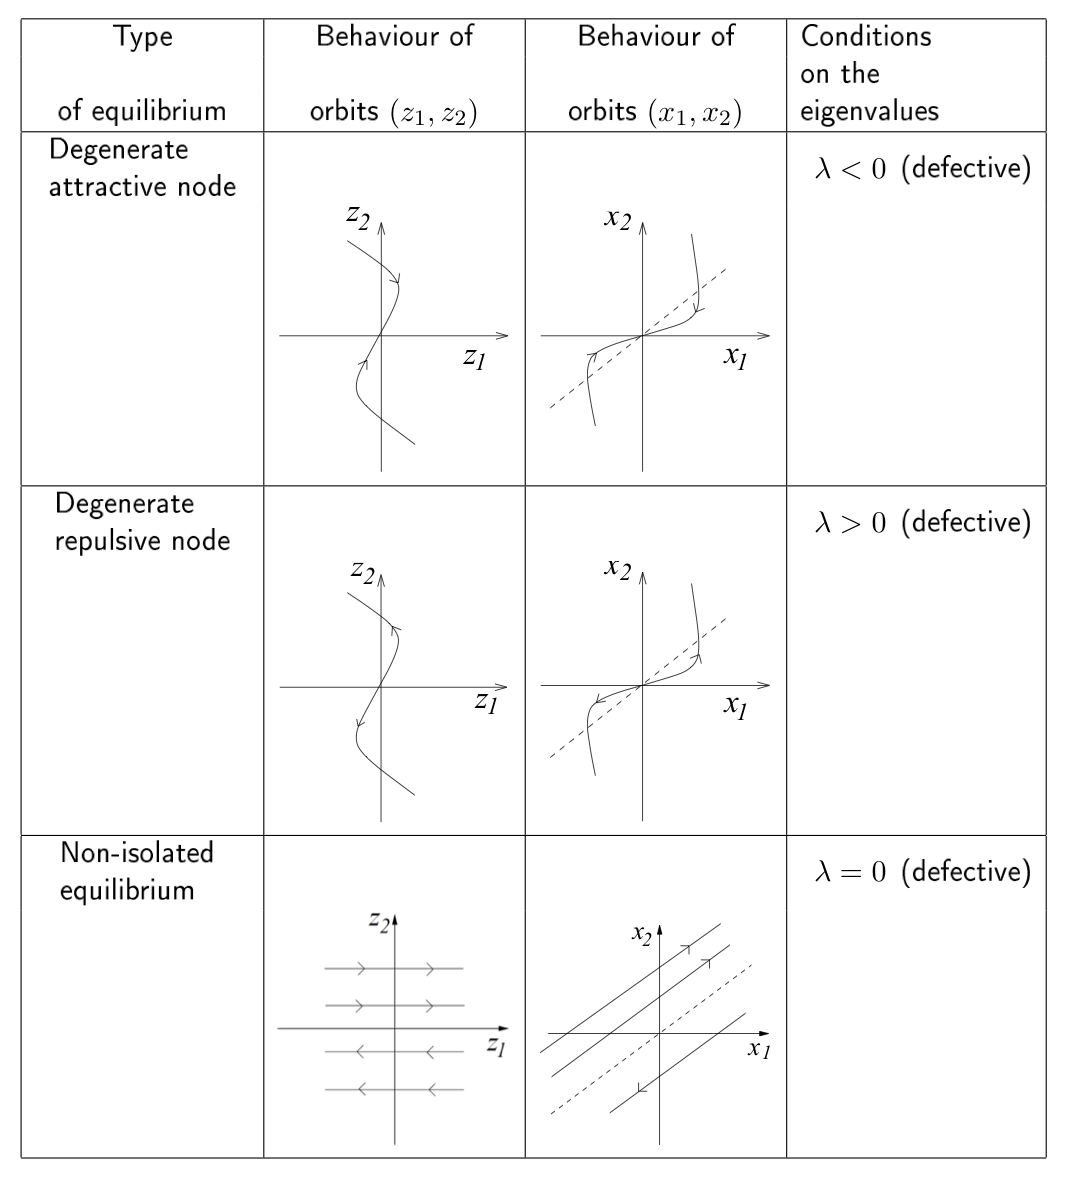
\includegraphics[width = \textwidth]{img/orbit_lin_sys_2.png}
\end{figure}
\begin{figure}[H]
    \centering
    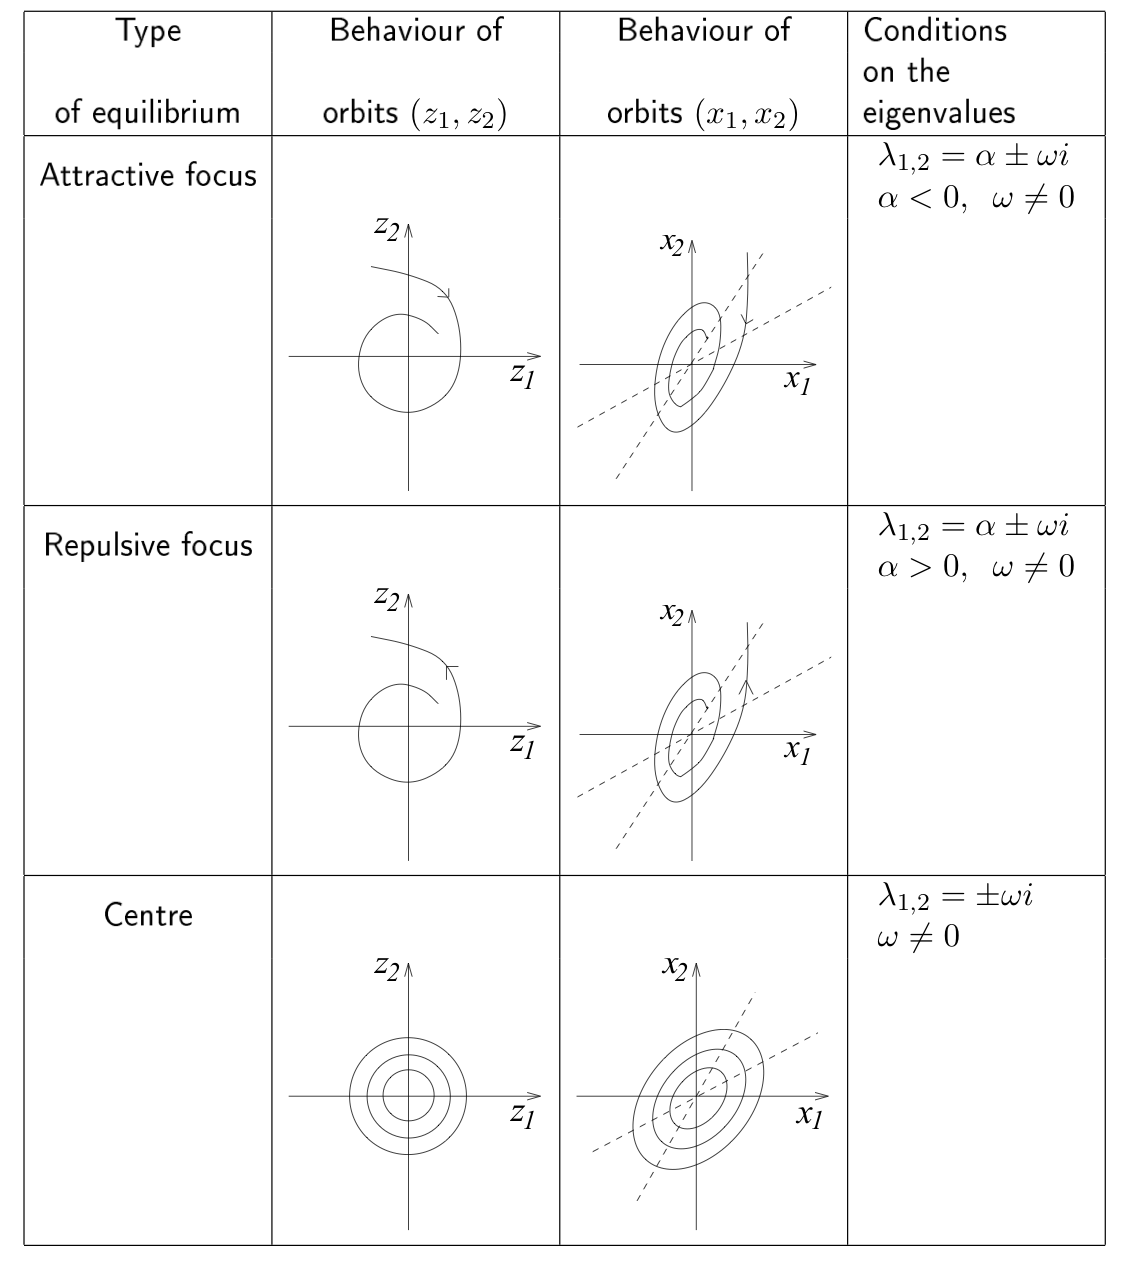
\includegraphics[width = \textwidth]{img/orbit_lin_sys_3.png}
\end{figure}
\begin{itemize}
    \item [\(\bullet\)] Note: if one of the eigenvalues is zero, the equilibrium is not isolated.
\end{itemize}
\begin{definition}
    If all trajectories of a linear system converge to an equilibrium, we say that it is an attractive equilibrium. It is a repulsive equilibrium if they all diverge to infinity (save for the equilibrium itself.)
\end{definition}
\begin{figure}[H]
    \centering
    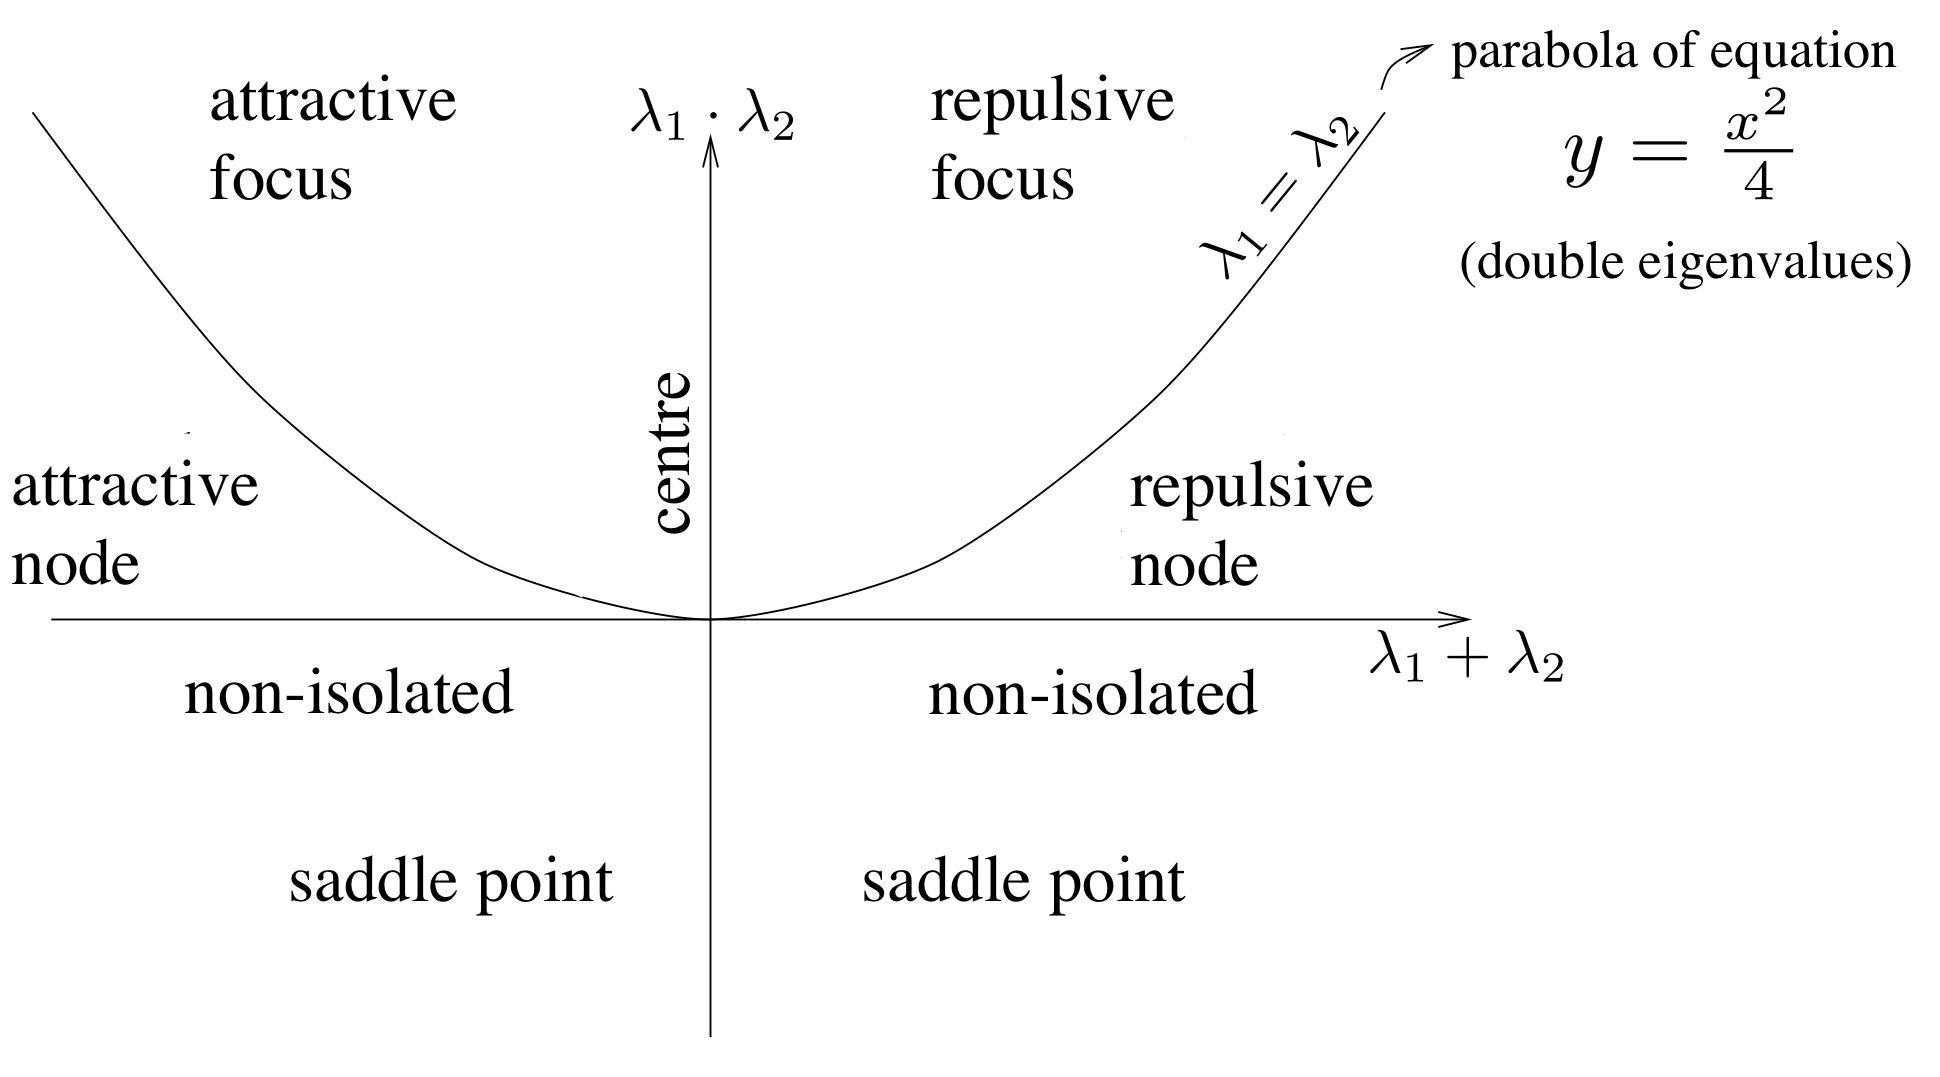
\includegraphics[width=.5\textwidth]{img/det_tr_2d.png}
\end{figure}
\begin{itemize}
    \item An attractive (resp. repulsive) equilibrium will remain attractive (resp.repulsive) after a perturbation and a saddle point will remain a saddle point. Such equilibria are called structurally stable. However, a center equilibrium (zero real part) is never structurally stable: even a small perturbation of the matrix \(A\) can shift eigenvalues away from the imaginary axis, and the corresponding trajectories then converge to the equilibrium or diverge from it.
\end{itemize}
\begin{definition}
    If all eigenvalues of \(A\) have nonzero real part, the equilibrium of \(\dot x=Ax\) is said to be hyperbolic.
\end{definition}
\section{Linearisation of nonlinear systems}
We assume the existence of an equilibrium \((\bar x, \bar u)\) for the nonlinear system \(\dot x = f(x,\bar u)\). The Taylor expansion is
\begin{equation}
    \dot x = f(\bar x,\bar u) + \left(\frac{\partial f(x,\bar u)}{\partial x}\right)_{\bar x}(x-\bar x)+\mathcal{O}(\lVert x-\bar x\rVert^2)
\end{equation}
Thus, the linear approximation of the system is, for \(\tilde x = x-\bar x\),
\begin{equation}\label{eq:linearisation}
    \dot{\tilde{x}} = \left(\frac{\partial f(x,\bar u)}{\partial x}\right)_{\bar x}\tilde x
\end{equation}
We define \(A\triangleq \left(\frac{\partial f(x,\bar u)}{\partial x}\right)_{\bar x}\) as the Jacobian matrix of \(f\) at the equilibrium.
\begin{definition}
    The equilibrium \((\bar x,\bar u)\) of the nonlinear system is said to be hyperbolic if all the eigenvalues of the jacobian matrix \(A\) have a nonzero real part. 
\end{definition}
\begin{definition}
    Two dynamical systems are topologically conjugate if there exists a homeomorphism, i.e. a continuous bijection whose inverse is also continuous, that maps the trajectories of the first system to the trajectories of the second one in a time respecting way. That means that the trajectories of \(\dot x = f(x)\) on a domain \(D\) and \(\dot y=g(y)\) on a domain \(E\) are topologically conjnugate through the homeomorphism \(\phi:D\rightarrow E\) if every curve \([0,t_0]\rightarrow D:t\rightarrow x(t)\) is a trajectory of the system \(f\) iff the corresponding curve \([0,t_0]\rightarrow E:t\rightarrow\phi(x(t))\) is a trajectory of the system \(g\).
\end{definition}
\begin{thm}
    If the equilibrium \((\bar x,\bar u)\) is hyperbolic, then the trajectories of the nonlinear system in a neighbourhood of the equilibrium \((\bar x,\bar u)\) are topologically conjugate to those of the linear approximation \eqref{eq:linearisation}. Specifically, there exists a neighbourhood \(X\) of \(\bar x\), a neighbourhood \(\tilde X\) of 0, and a homeomorphism \(\phi:X\rightarrow\tilde X\) with \(\phi(\bar x)=0\) such that if \(t\rightarrow x(t)\) is a trajectory of the nonlinear system contained in \(X\), then \(t\rightarrow \phi(x(t))\) is a trajectory of the linear system.
\end{thm}
That means that if the equilibrium is a node/focus (attractive or repulsive) or a saddle point (but not a centre) in the linearised system, then the linearised system is a good representation for the local behaviour of the nonlinear trajectories around the equilibrium as well. However, this theorem is local, and the higher-order terms are needed to conclude in the case of a non-hyperbolic equilibrium. 
\chapter{Bifurcations}
Bifurcation theory looks at the impact of the value \(\bar u\) on the nature and number of equilibria. 
\section{Hopf bifurcation}
\begin{figure}[H]
    \centering
    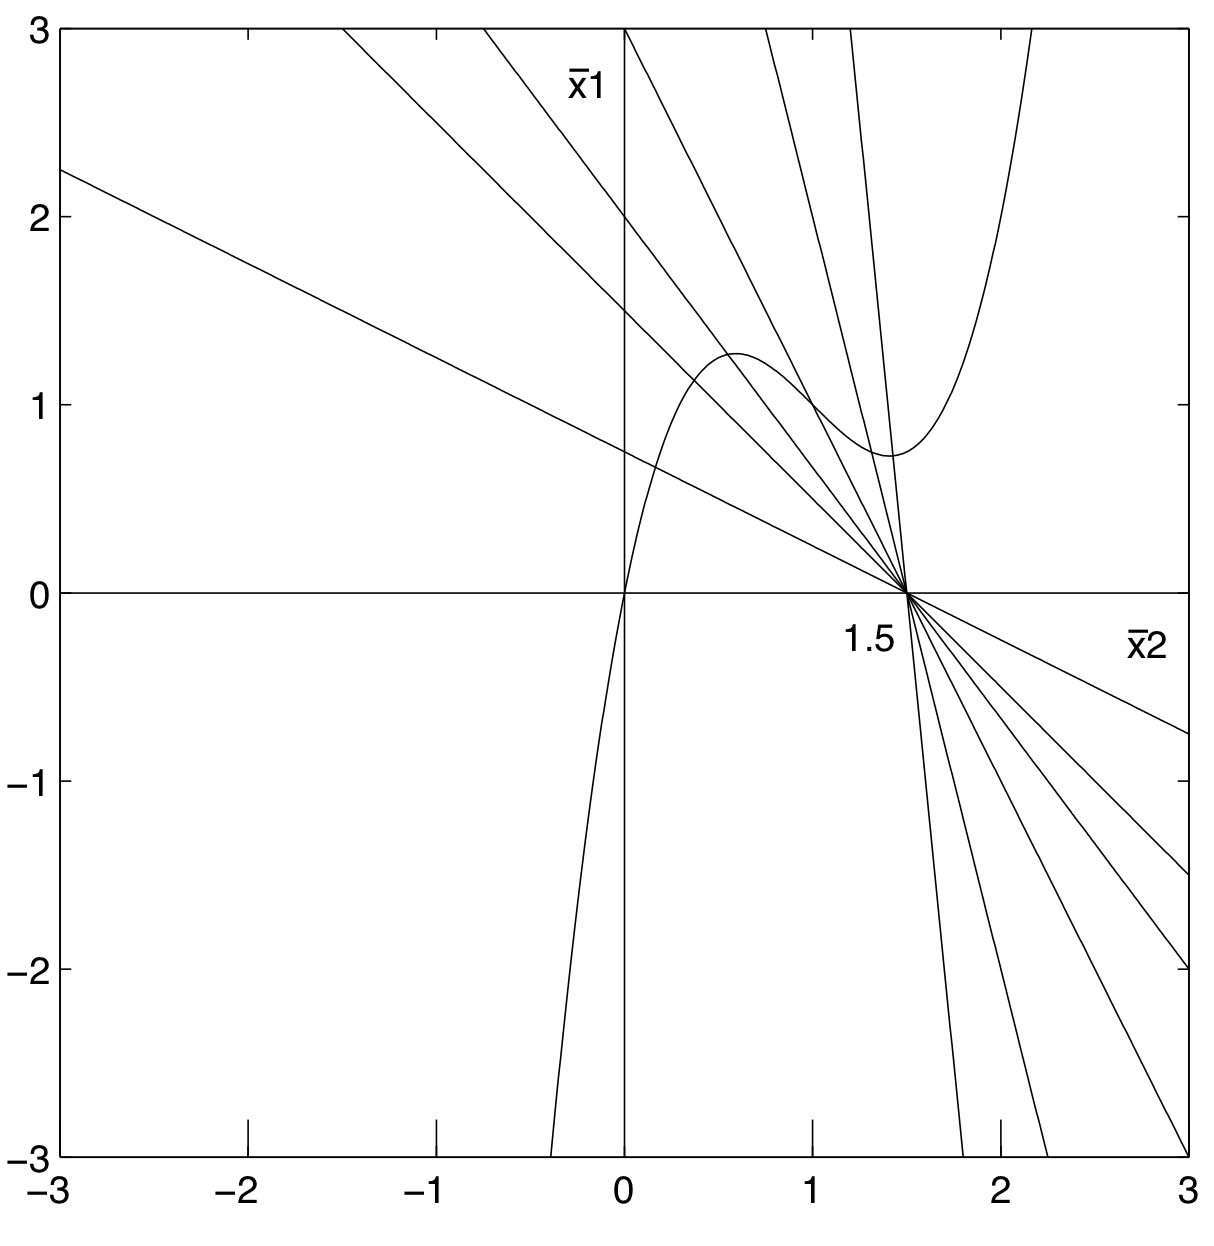
\includegraphics[width = .4\textwidth]{img/hopf_bif.png}
\end{figure}
Depending on the slope of the straight line, the characterization of the equilibrium changes: it is an attractive focus, then changes to repulsive focus and goes back to being an attractive focus.
\begin{thm}
    Suppose that a system has a family of isolated equilibria \((\bar x,\bar u)\) parametrized by \(\bar u\). Suppose that there exists a value \(\bar u^*\) such that a pair of eigenvalues of the Jacobian matrix evaluated in this equilibrium have a zero real part and a nonzero imaginary part. These values depend continuously on \(\bar u\), at least in the neighbourhood of \(\bar u^*\), and are denoted by
\end{thm}
\begin{equation}
    \lambda_i(\bar u) = \alpha(\bar u)\pm i\omega(\bar u)
\end{equation}
Suppose also that \(\frac{d\alpha (\bar u^*)}{d\bar u}>0\). Thus, for \(\bar u\) close enough to \(\bar u^*\), the equilibrium is attractive for \(\bar u<\bar u^*\) and repulsive for \(\bar u>\bar u^*\). \\
Then, there generically exists either an attractive closed orbit (i.e. limit cycle) for all \(\bar u^*<\bar u<\bar u^*+\varepsilon\) or a repulsive closed cycle for \(\bar u^*-\varepsilon < \bar u < \bar u^*\) (for some \(\varepsilon>0\)) unique in the neighbourhood of the equilibrium.
\section{Transcritical bifurcation}
\begin{figure}[H]
    \centering
    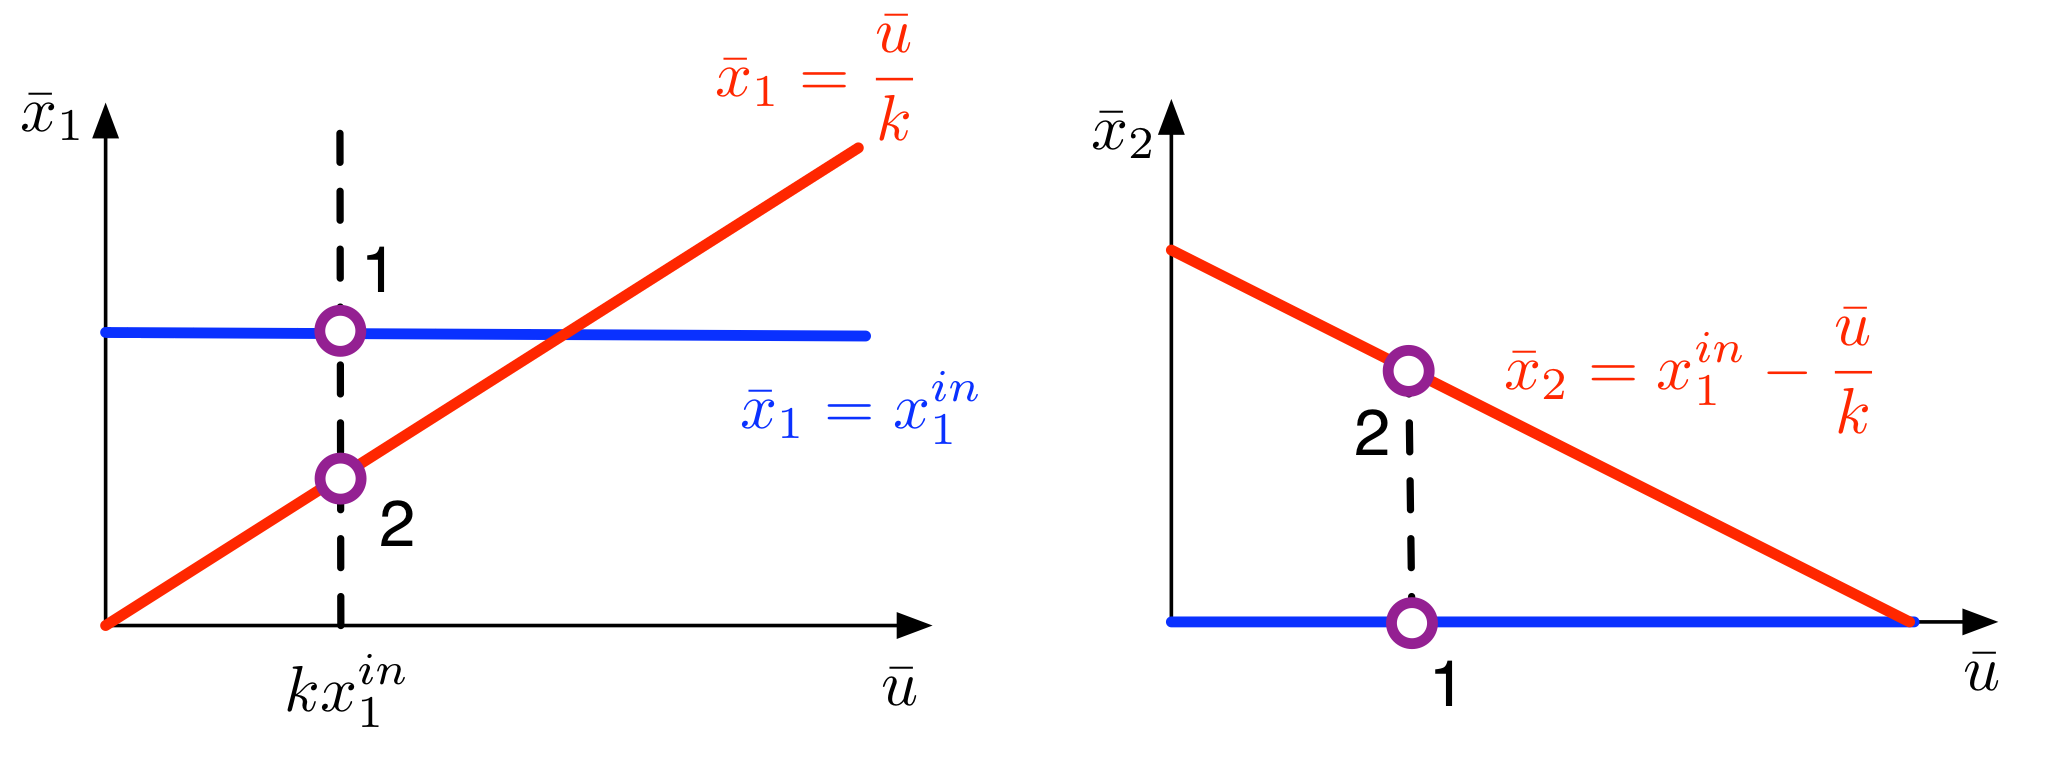
\includegraphics[width = .5\textwidth]{img/transcritical.png}
\end{figure}
In this example, the first equilibrium is attractive if \(\bar u>kx_1^{in}\) and is a saddle point otherwise. The second however is a saddle point when the above condition is met and attractive when it is not.\\

A transcritical bifurcation is thus such that the characterization of the two equilibria switch when passing a certain threshold value of \(\bar u\).
\section{Saddle-node/Fold bifurcation}
For small values of \(\bar u\), the system has a single equilibrium. Then, for a critical value of \(\bar u\), the system exhibits two more equilibrium values (one a saddle point and the other attractive). By further increasing \(\bar u\), we cross a new critical value beyond which the system has only a single equilibrium that is also attractive. \\
\begin{figure}[H]
    \centering
    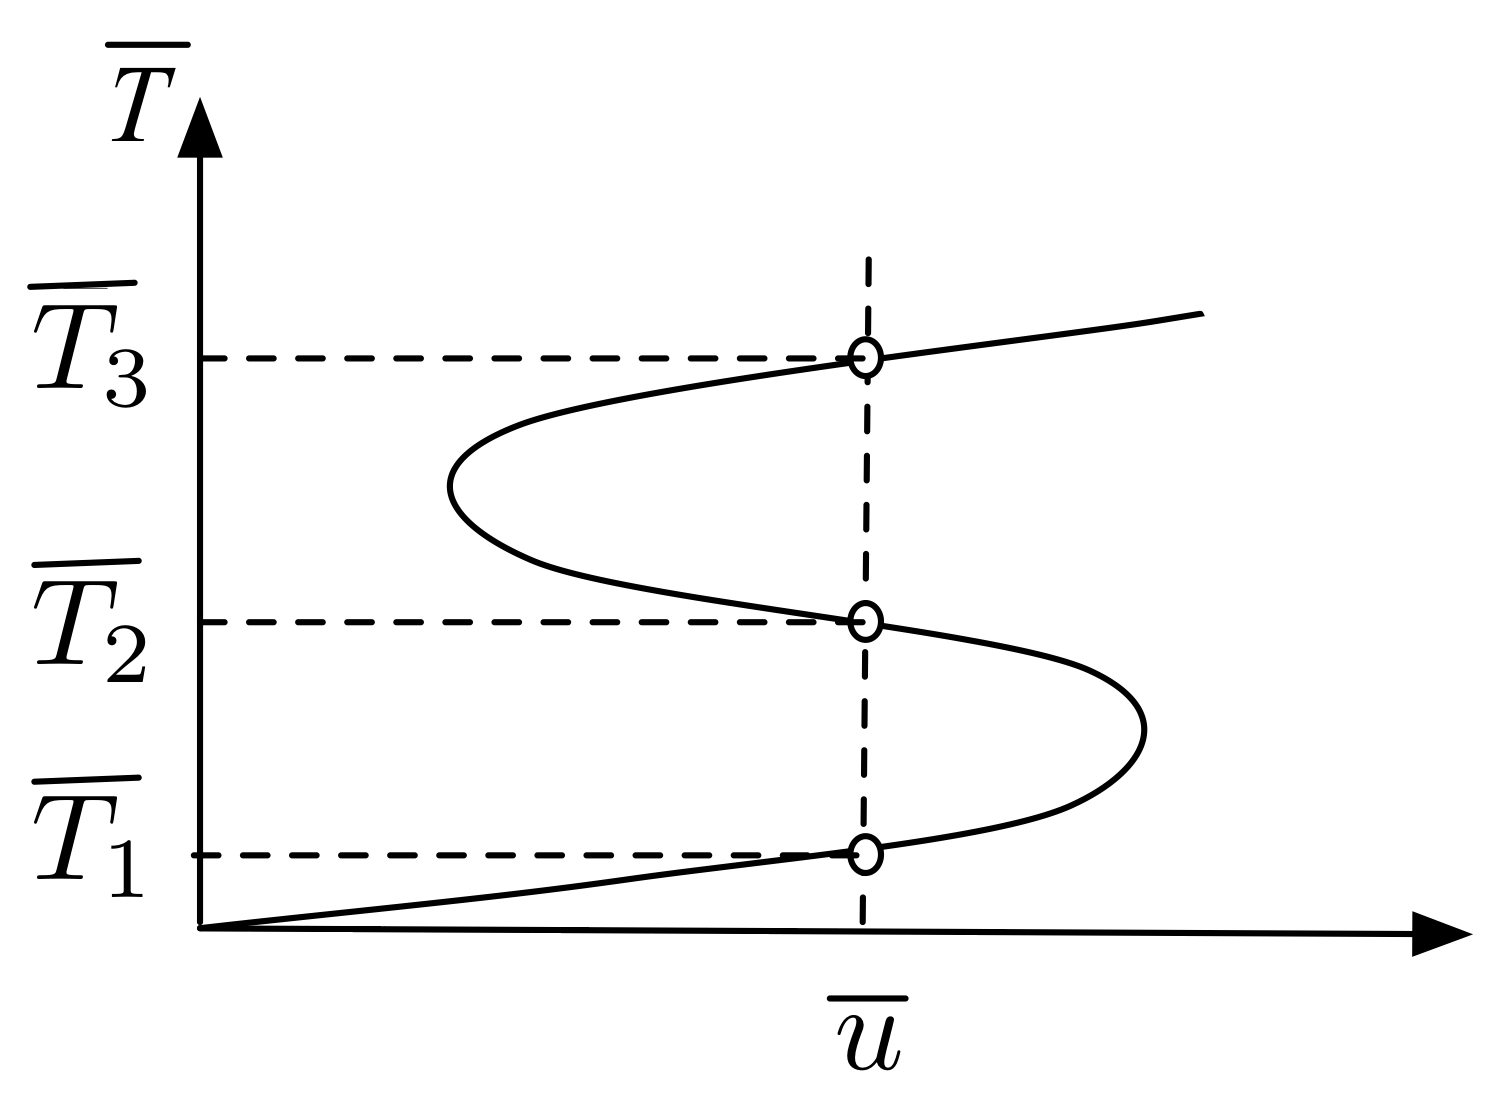
\includegraphics[width = .3\textwidth]{img/fold_bif.png}
\end{figure}
As the input \(\bar u\) is slowly modified from low to high values, the state of the system, initially following the bottom line of equilibria, goes through a brutal change at the rightmost bifurcation, where it jumps to a different equilibrium. It is called a catastrophe. As the input decreases again to low values, the catastrophe happens the other way. This is a hysteresis.
\section{Pitchfork bifurcation}
A pitchfork bifurcation is the split, for some value \(\bar u^*\) of the birufcation parameter, of a single attractive (resp. repulsive) equilibrium into three equilibria, one being repulsive (resp. attractive) and the other two being attractive (resp. repulsive). 
\begin{figure}[H]
    \centering
    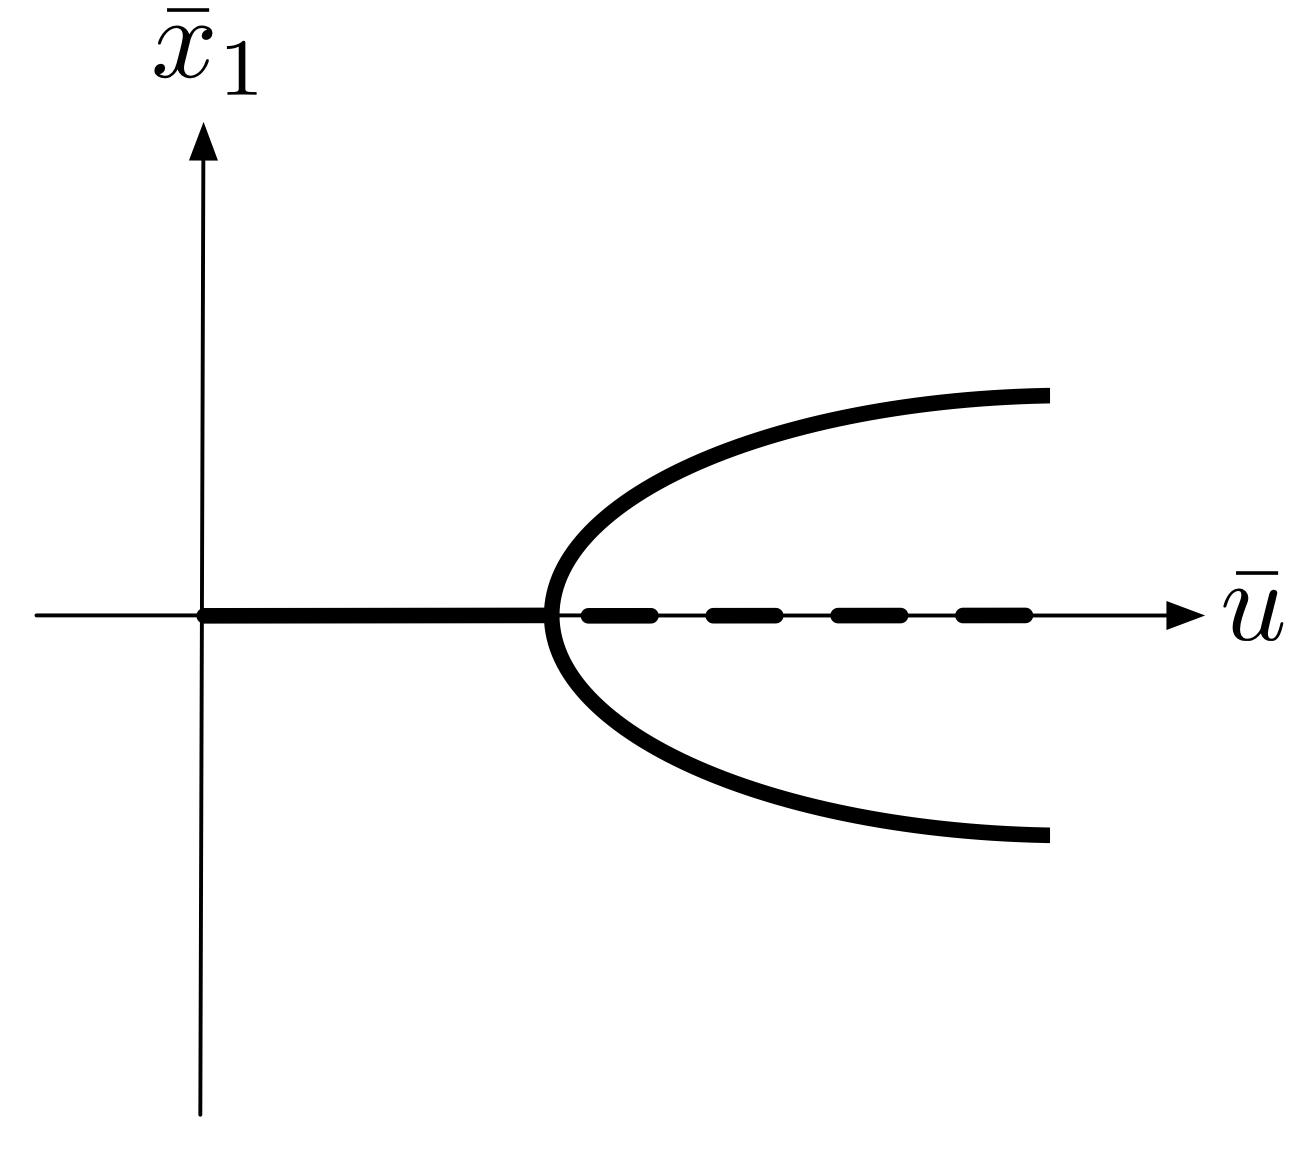
\includegraphics[width = .4\textwidth]{img/pitchfork_bif.png}
\end{figure}
\chapter{Stability of equilibria}
In this chapter we assume that the locally Lipschitz continuous vector field \(f(\cdot,\bar u)\) is defined on an open set \(\Omega\subseteq\R^n\) for a fixed value of \(\bar u\), where the trajectories are defined and stay in \(\Omega\) for all positive times. 
\section{Definitions}
\begin{definition}
    The equilibrium \((\bar x,\bar u)\) is said to be stable if \begin{equation}
        \forall \varepsilon>0, \exists \delta>0 \text{ such that } \forall x_0\in \Omega:\: \lVert x(t_0)-\bar x\rVert <\delta \Longrightarrow \lVert x(t,x(t_0), \bar u)-\bar x\rVert<\varepsilon \quad \forall t\ge t_0
    \end{equation}
\end{definition}
That means that an equilibrium is stable if the trajectories remain arbitrarily close to it, provided that they start close enough from this equilibrium. 
\begin{definition}
    The equilibrium \((\bar x,\bar u)\) is said to be attractive if \begin{equation}
        \exists \delta >0\text{ such that } \lVert x(T_0)-\bar x\rVert <\delta \Longrightarrow \lim_{t\rightarrow \infty} \lVert x(t,x(t_0),\bar u)-\bar u\rVert=0
    \end{equation}
\end{definition}
An attractive equilibrium \(\bar x\) is thus a point to which each solution \(x\) converges provided that it starts close enough to \(\bar x\). 
\begin{itemize}
    \item [\(\rightarrow\)] Note: stability and attractiveness do not imply each other.
\end{itemize}
\begin{definition}
    The equilibrium \((\bar x,\bar u)\) is said to be asymptotically stable if it is both stable and attractive. The set of points \(x_0\) for which the trajectory \(x(t,x_0, \bar u)\) converges to \(\bar x\) is called the basin of attraction of the saymptotically stable equilibrium. 
\end{definition}
\begin{definition}
    The equilibrium \((\bar x,\bar u)\) is said to be exponentially stable if \begin{equation}
        \exists a,b,\delta>0 \text{ such that }\lVert x(t_0)-\bar x\rVert <\delta \Longrightarrow \lVert x(t,x(t_0),\bar u)-\bar x\rVert \le a\lVert x(t_0)-\bar x\rVert e^{-bt}\qquad \forall t\ge t_0
    \end{equation}
\end{definition}
\begin{itemize}
    \item [\(\rightarrow\)] Note: exponential stablity implies asymptotic stability.
    \item [\(\rightarrow\)] Note: for a linear system, an attractive equilibrium and center are both stable, while a saddle or repulsive equilibrium is unstable. Attractive equilibrium is also exponentially stable, thus asymptotically stable: these three notions coincide for linear systems. 
\end{itemize}
\section{Lyapunov's first method}
\begin{thm}
    \begin{itemize}
        \item If the equilibrium is attractive in the linearised system, i.e. all eigenvalues of the Jacobian matrix have a negative real part, then the equilibrium \((\bar x,\bar u)\) is exponentially stable.
        \item If the equilibrium is repulsive or a saddle point in the linearised system, i.e. the Jacobian matrix has at least one eigenvalue with a positive real part, then the equilibrium \((\bar x,\bar u)\) is unstable. 
    \end{itemize}
\end{thm}
This theorem does not conclude on the stability of a non-hyperbolic equilibrium. 
\section{Lyapunov's second method}
\begin{thm}
    The equilibrium \((\bar x,\bar u)\) of the system \(\dot x=f(x,\bar u)\), where \(f\) is locally Lipschitz continuous on an open set \(\Omega \subseteq \R^n\) is stable if there exists a continuously differentiable function \(V:\Omega\rightarrow \R\) with the following properties:
    \begin{itemize}
        \item \(\Omega\subseteq \R^n\) is a neighbourhood of \(\bar x\);
        \item \(V(x)>V(\bar x) \: \forall x\in \Omega \setminus \{\bar x\}\), i.e. \(V\) has a strict minimum point at \(\bar x\);
        \item \(\dot V(x)\le 0\:\forall x\in \Omega \setminus\{\bar x\}\).
    \end{itemize}
\end{thm}
That means that a sufficient condition for the equilibrium \((\bar x,\bar u)\) to be stable is to have a positive-definite function \(V-V(\bar x)\) whose temporal derivative \(\dot V\) along trajectories is negative-semidefinite in a neighbourhood of \(\bar x\), the temporal derivative being defined as 
\begin{equation}
    \dot V(x) = \frac{dV}{dt} = \frac{\partial V}{\partial x} \dot x = \sum_{i=1}^n \frac{\partial V}{\partial x_i}f_i(x,\bar u) = \langle \nabla V(x(t)),f(x(t),\bar u)\rangle
\end{equation}
\begin{thm}
    The equilibrium \((\bar x,\bar u)\) of the system \(\dot x = f(x,\bar u)\) is asymptotically stable if there exists a continuously differentiable function \(V:\Omega\rightarrow\R\) with the following properties:
    \begin{itemize}
        \item \(\Omega \subseteq \R^n\) is a neighbourhood of \(\bar x\);
        \item \(V(x)>V(\bar x) \: \forall x\in \Omega \setminus\{\bar x\}\), i.e. \(V\) has a strict global minimum point at \(\bar x\);
        \item \(\dot V(x)<0\: \forall x\in \Omega\setminus \{\bar x\}\).
    \end{itemize}
\end{thm}
\begin{thm}
    The basin of attraction of an asymptotically stable equilibrium is an open, connected, invariant set; and its boundary is formed by trajectories.
\end{thm}
\begin{definition}
    Let \(f:\R^N\rightarrow \R^N\) be locally Lipschitz continuous and \(\bar x\in \R^N\) be an equilibrium of \(f\). The equilibrium \(\bar x\) is said to be globally asymptotically stable if it is asymptotically stable and its basin of attraction is the whole state spce \(\R^N\). 
\end{definition}
\begin{definition}
    A function \(V:\R^N\rightarrow \R\) is said to be radially unbounded if \(\lVert x\rVert \rightarrow \infty\) implies \(V(x)\rightarrow \infty\), i.e. for every \(M\in\R\), there exists \(R\ge 0\) such that, for every \(x\in \R^N\), \(\lVert x\rVert \ge R\) implies \(V(x)\ge M\). 
\end{definition}
\begin{thm}
    Let \(f:\R^N\rightarrow \R^N\) be locally Lipschitz continuous and \(\bar x\in \R^N\) be an equilibrium of \(f\). If there exists a radially unbounded continuously differentiable function \(V:\R^N\rightarrow \R\) such that, for every \(x\in \R^N\setminus \{\bar x\}\), \(V(x)>V(\bar x)\) and \(\dot V_f(x)<0\), then \(\bar x\) is globally asymptotically stable.
\end{thm}
\subsection{LaSalle's invariance principle}
\begin{definition}
    A function \(x:\R^+\rightarrow\R^N\) is said to asymptotically approach a nonempty set \(M\subseteq \R^N\) if 
    \begin{equation}
        \lim_{t\rightarrow \infty} \underbrace{\inf_{y\in M} \lVert x(t)-y\rVert}_{\eqcolon \text{dist}(x(t),M)} = 0
    \end{equation}
\end{definition}
\begin{thm}
    Let \(F\subseteq \Omega\) be a compact (positively) invariant set for \(f\). Let \(V:\Omega \rightarrow \R\) be a continuously differentiable and such that \(\dot V_f \le 0\) for every \(x\in F\). Let \(E\coloneqq \{x\in F|\dot V_f (x)=0\}\). Let \(M\) be the largest (positively and negatively) invariant set in \(E\). Then, every trajectory of \(f\) starting in \(F\) asymptotically approaches \(M\). 
\end{thm}
\begin{crl}
    Let \(\bar x\) be an equilibrium of \(f\). Let \(V:\Omega\rightarrow \R\) be continuously differentiable and such that, for every \(x\in \Omega\setminus \{\bar x\}\), \(V(x)>V(\bar x)\) and \(\dot V(x)\le 0\). Let \(S\coloneqq \{x\in \Omega |\dot V(x)=0\}\). If the equilibrium is the only trajectory fully contained (past and future) in \(S\), then \(\bar x\) is asymptotically stable. 
\end{crl}
\section{The energy as a Lyapunov function}
\begin{itemize}
    \item [\(\rightarrow\)] Note: the Lyapunov function \(V(x)\) often has the dimensions of an energy. 
\end{itemize}
\subsection{In mechanical systems}
The general equation in a mechanical system\footnote{See chapter \ref{sec:mechanical}} is 
\begin{equation}
    M(q)\ddot q + C(q,\dot q)\dot q+g(q)+k(q)+h(\dot q)=G\bar u
\end{equation}
Here we assume the kinematic matrix \(G\) to be constant. The Lyapunov function taken for this general system is 
\begin{align}
    V(q,\dot q) &= \frac{1}{2}\dot q^TM(q)\dot q+E_p(q)-q^TG\bar u\\
    \dot V(q,\dot q) &= -\dot q^Th(\dot q)
\end{align}
The first term is the kinetic energy, the second is the potential energy and the third is the work realized by the applied forces and torques.
\subsection{In electrical systems}
For electrical systems, there isn't a general formula of the state-space model. The Lyapunov function will however still have the dimensions of an energy, with different terms:
\begin{itemize}
    \item Inductance: \(E = \frac{1}{2}Li^2\)
    \item Capacitance: \(E = \frac{1}{2}Cv^2\)
    \item Resistance: \(E = Ri^2\)
\end{itemize}
\section{Linear systems}
Let us study once again the system \eqref{eq:linear_sys} with an equilibrium \((\bar x,\bar u)\). We define the Lyapunov function \[V(x) = (x-\bar x)^TP(x-\bar x)\] where \(P\) is a symmetric positive-definite matrix. Its derivative is \(\dot V(x) = -(x-\bar x)^TQ(x-\bar x)\), with \(-Q=A^TP+PA\). 
\begin{align}
    V(x) &= (x-\bar x)^TP(x-\bar x)\\
    \dot V(x) &= -(x-\bar x)^TQ(x-\bar x)\qquad -Q = A^TP+PA \label{eq:lyapunov}
\end{align}
\begin{thm}
    Let \(A\) be a real matrix of order \(n\). For every positive-definite matrix \(Q\), equation \eqref{eq:lyapunov} owns a unique positive-definite solution \(P\) iff \(A\) is a Hurwitz matrix, i.e. all its eigenvalues have a negative real part.
\end{thm}
\section{Bounded-input, bounded-state stability}
We are here interested in an input signal \(u(t)\) that is bounded and close to \(\bar u\). We need to analyse this case because a constant signal is not feasible in reality. We study the linear system
\begin{equation}
    \dot x = Ax+Bu \quad x(t_0) = x_0
\end{equation}
The trajectory of the system is
\begin{equation}
    x(t) = e^{A(t-t_0)}x_0 + \int_{t_0}^t e^{A(t-\tau)}Bu(\tau)d\tau
\end{equation}
The equilibrium is \((\bar x,\bar u)= (0,0)\). It is asymptotically stable iff the matrix \(A\) is a Hurwitz matrix. This would mean that \(\lVert e^{At}\rVert\) is bounded for all \(t\ge t_0\) and there are nonnegative constants \(k\) and \(\lambda\) such that 
\begin{equation}
    \lVert e^{A(t-t_0)}\rVert \le ke^{-\lambda(t-t_0)}
\end{equation}
and thus
\begin{equation}
    \lVert x(t)\rVert \le ke^{-\lambda (t-t_0)}\lVert x_0\rVert + \frac{k\lVert B\rVert}{\lambda}\sup_{t_0\le \tau\le t}\lVert u(\tau)\rVert
\end{equation}
This means that a bounded input \(u(t)\), however big its magnitude is, generates a bounded state \(x(t)\), and the effect of the initial condition \(x_0\) fades away with time. 
\begin{thm}
    If the equilibrium \((\bar x, \bar u)\) of the linear system is asymptotically stable,
    \begin{itemize}
        \item there are three nonnegative constants \(c_1,c_2,c_3\) such that, for each initial state \(x_0\) with \(\lVert x_0-\bar x\rVert<0\) and each input signal \(u\) with \(\lVert u(t)-\bar u\rVert <c_2\) \(\forall t\ge t_0\), the solution \(x\) is bounded: \(\lVert x(t)-x_0\rVert <c_3\) \(\forall t\ge t_0\);
        \item there is a nonnegative constant \(c_0\) and a continuous function \(\alpha :[0,a)\rightarrow [0,\infty)\) passing through the origine, i.e. \(\alpha(0)=0\), and increasing such that, for each input signal \(u\) with \(\lVert u(t)-\bar u\rVert<c_0\) \(\forall t\ge t_0\), the ultimate bound on \(x\) is an increasing function of the bound on \(u\) :
    \end{itemize}
    \begin{equation}
        \lim_{t\rightarrow \infty}\sup \lVert x(t)\rVert \le \alpha(\lVert u\rVert_{\mathcal{L}_{\infty}})
    \end{equation}
\end{thm}
\begin{thm}
    If \(f\) is globally continuously differentiable and globally Lipschitz continuous, and if the equilibrium \((\bar x,\bar u)\) is globally exponentially stable, then for each initial condition \(x_0\), and each input signal \(u\), the solution \(x\) is bounded.
\end{thm}
\chapter{Controllability and trajectory planning}\label{chap:11}
\begin{definition}
    For the dyanmical system \(\dot x=f(x,u)\), the final state \(x_f\in \R^n\) is reachable from the initial state \(x_0\in \R^n\) within time \(T\) if there exists an input function \(u:[t_0,t_0+T]\rightarrow \R^m\) such that \(x(t_0)=x_0\) and \(x(t_0+T)=x_f\).
\end{definition}
\section{Controllability of LTI systems}
\begin{definition}
    The system \(\dot x = Ax + Bu\), for \(x\in \R^n\) and \(u\in \R^m\), is controllable if, for each initial state \(x_0\), it is possible to reach any other final state \(x_f\) within any positive time \(T\).
\end{definition}
\begin{thm}
    The LTI system \(\dot x=Ax+Bu\) is completely controllable iff one of the two following criteria is satisfied:
    \begin{itemize}
        \item The matrix \(\mathcal{C}=\begin{bmatrix}
            B & AB & A^2B & \cdots & A^{n-1}
        \end{bmatrix}\) has full rank;
        The rank of the matrix \(\begin{bmatrix}
            sI-A & B
        \end{bmatrix}\) is equal to \(n\) for each \(s\in \C\)
    \end{itemize}
\end{thm}
If the controllability matrix has rank \(d<n\), we define a matrix \(T = (T_a\: T_b)\) such that \(T_a\) contains \(d\) linearly independent columns of \(\mathcal{C}\) and \(T_b\) completes the matrix by \(n-d\) vectors independent of the columns of \(T_a\). Its inverse is \(T^{-1}\coloneqq \begin{pmatrix}
    U_a \\ U_b
\end{pmatrix}\), where the matrices \(U_a,U_b\) are chosen such that 
\begin{equation}
    T^{-1}T = \begin{pmatrix}
        U_aT_a & U_aT_b \\ U_bT_a & U_bT_b\\
    \end{pmatrix} = \begin{pmatrix}
        I_d & 0 \\ 0 & I_{n-d}\\
    \end{pmatrix}
\end{equation}
From that, we define a state transformation 
\begin{equation}
    z = \begin{pmatrix}
        z_a \\ z_b\\
    \end{pmatrix} = \begin{pmatrix}
        U_ax & U_bx\\
    \end{pmatrix}
\end{equation}
The new state-space model is 
\begin{align}
    \dot z_a &= U_aAT_az_a + U_aAT_bz_b + U_aBu\\
    \dot z_b &= U_bAT_bz_b
\end{align}
The part \(z_b\) is the non controllable part of the system, it is not influenced by the input \(u\).
\section{Controllability of nonlinear systems}
\begin{definition}
    The system \(\dot x = f(x,u)\) for \(x\in \R^n\) and \(u\in \R^m\) is locally accessible from the initial state \(x_0\) if for any time \(T\), the set of states reachable from \(x_0\) within \(T\) contains a nonempty open set.
\end{definition}
\begin{definition}
    The system \(\dot x=f(x,u)\) for \(x\in \R^n\) and \(u\in \R^m\) is locally controllable from the initial state \(x_0\) if for any time \(T\), the set of states reachable from \(x_0\) within \(T\) contains a neighbourhood of \(x_0\). 
\end{definition}
We can also define the global controllability, which requires that the whole state space is reachable from any initial condition. 
\begin{itemize}
    \item [\(\rightarrow\)] Note: local accessibility, local controllability and global controllability are equivalent for linear systems.
\end{itemize}
\section{Drawbacks of linearisation}
\begin{thm}
Let us consider the linearisation of the system \(\dot x=f(x,u)\) around an equilibrium\((\bar x,\bar u)\): 
\begin{equation}
    \dot x = Ax+Bu \qquad A= \left(\frac{\partial f}{\partial x}\right)_{(\bar x,\bar u)} \qquad B = \left(\frac{\partial f}{\partial u}\right)_{(\bar x,\bar u)}
\end{equation}
If the linearised system is controllable, then for each \(\varepsilon >0\), the set of states reachable from \(\bar x\) within time \(T\) with inputs \(u(t)\) such that \(\lVert u(t)-\bar u\rVert <\varepsilon \), contains a neighbourhood of \(\bar x\).
\end{thm}
We now define a new operator, the Lie bracket of two vector fields:
\begin{equation}
    [g_1,g_2] \coloneqq \frac{\partial g_2}{\partial x}g_1-\frac{\partial g_1}{\partial x}g_2
\end{equation}
\begin{thm}
    Let us consider the control-linear system\footnote{Control-linear means linear in every input.} in some open set \(X\subseteq \R^n\):
    \begin{equation}
        \dot x= g_1(x)u_1 + \dots + g_m(x)u_m
    \end{equation}
    for some analytic\footnote{Analytic means that all coordinates of all fields \(g_i\) have a Taylor series that converges in a neighbourhood, i.e. all derivatives of all order exist.} vector fields \(g_1,\dots,g_m\). Consider the set of all vector fields \(g_1,\dots,g_m\) and their repeated Lie brackets. Consider also the vector space generated by all these vector fields evaluated at a state \(x_0\). This vector space is of dimension \(n\) iff the system is locally controllable from \(x_0\). Moreover, if this condition is met everywhere in the state space \(X\), then the system is globally controllable.
\end{thm}
\begin{thm}
    Let us consider the system in \(X\subseteq \R^n\):
    \begin{equation}
        \dot x=f(x)+g_1(x)u_1 + \dots + g_m(x)u_m
    \end{equation}
    for some analytic vector fields \(f,g_1,\dots,g_m\). Consider the set of all vector fields \(f,g_1,\dots,g_m\) and those obtained by repeated Lie brackets. Consider also the vector space generated by those vector fields evaluated at a state \(x_0\). This vector space is of dimension \(n\) iff the system is locally accessible from \(x_0\).
\end{thm}
\section{Trajectory planning}
We work here with the following Brunovsky form of the nonlinear system:
\begin{align}
    \dot z_1 &= z_2 \nonumber\\
    \dot z_2 &= z_3 \nonumber\\
    &\vdots \nonumber\\
    \dot z_n &= \alpha(z) + \beta(z)u \qquad \beta(z)\neq 0 
\end{align}
It is sufficient to define a polynomial trajectory for \(z_1\):
\begin{equation}
    z_1(t) = \sum_{i=0}^{2n-1}\lambda_i \left(\frac{t}{T}\right)^i
\end{equation}
By calculating the successive derivatives of \(z_1(t)\), we obtain the expressions of \(z_j(t)\), for \(j=2,\dots,n\):
\begin{equation}
    z_j(t) = \sum_{i=j-1}^{2n-1}\frac{i!}{(i-j+1)!}\frac{\lambda_i}{T^{j-1}}\left(\frac{t}{T}\right)^{1-j}
\end{equation}
and we can find the values of coefficients \(\lambda_i\) by calculating those values for \(t=0\) and \(t=T\). Finally, the input we need to obtain the wanted results is 
\begin{equation}
    u(t) = \frac{\dot z_n(t)-\alpha(z(t))}{\beta(z(t))}
\end{equation}
\chapter{Exercises}
\section{Electrical systems}
The three main components are 
\begin{itemize}
    \item Resistance : $v=Ri$, does not induce an ODE.
    \item Capacitance : $q=CV\rightarrow i_c = C\frac{dV_C}{dt}$
    \item Inductance : $v_L = L\frac{di_L}{dt}$
\end{itemize}
The graph of the circuit is such that every component is an edge and every cable connecting them is a node. We have $M$ edges and $N$ nodes.
\subsection{Resolution method}
\begin{itemize}
    \item Draw the graph of the circuit;
    \item Write the equations with Kirchhoff's laws, they give $N-1$ current equations and $M+1-N$ voltage equations;
    \item Simplify equations;
    \item Write the final system.
\end{itemize}
A capacitance mesh is a mesh of more than 2 capacitances. \\
An inductance cut is a node with more than 2 inductances. 
\section{Mechanical systems}\label{sec:mechanical}
\subsection{For a single body}
For a single body, we first set an arbitrary orthonormal inertial basis. The position of the body is characterized by its coordinates and its orientation:
\begin{equation}
    q \coloneqq \begin{pmatrix}
        x\\y\\\theta
    \end{pmatrix}
\end{equation}
The equations we use for the ODE system are
\begin{align}
    m\ddot x &= F_x\\
    m\ddot y &= F_y\\
    I\ddot \theta &= T
\end{align}
Where $m$ is the mass of the body, $I$ its moment of inertia, $F_x,F_y$ the forces applied to the body, and $T$ the resultant of the torques. \\
The final equation to solve for that system is 
\begin{equation}
    J\ddot q+b(q) = B(q)u
\end{equation}
where $J$ is the diagonal and constant inertia matrix, $b(q)$ represents the effect of the gravity, $B(q)$ is a the kinematic matrix which depends nonlinearly on the state variables, and $u$ contains the input variables, e.g. some forces applied to the body. The state-space model is thus 
\begin{align}
    \dot q&= v \nonumber \\
    \dot v &= J^{-1}(-b(q)+B(q)u)
\end{align}
\subsection{Articulated mechanical systems}
\underline{General procedure:}
\begin{itemize}
    \item Choose an inertial basis and $N$ moving frames attached to the centers of mass of the $N$ bodies:
\end{itemize}
We get a vector of dimension $3N$:
\begin{equation}
    \xi = (x_1, y_1,\theta_1,\dots, x_N,y_N,\theta_N)^T
\end{equation}
\begin{itemize}
    \item Write the expressions of the constraints to which the motion of the system is subjected:
\end{itemize}
The algebraic relations are written such that 
\begin{equation}
    \Phi(\xi)=0
\end{equation}
where $\Phi:\Omega \rightarrow \R^p$ is a $\mathcal{C}^1$ mapping, and $p$ is the number of constraints. We choose a partition $\xi = (q,\bar q)$ such that the dimension $\sigma$ of $\bar q$ is equal to the rank of the Jacobian matrix of the mapping $\Phi$:
\begin{equation}
    \sigma \coloneqq \text{dim}(\bar q)= \text{rank}\frac{\partial \Phi}{\partial \xi}
\end{equation}
and such that we can express $\bar q$ as a function of $q$: $\bar q=\phi(q)$. This removes the redundant coordinates $\bar q$ of the system description. The number of degrees of freedom is thus $\delta\coloneqq 3N-\sigma$. 
\begin{itemize}
    \item Write the equations of motion for each coordinate with the Lagrange method:
\end{itemize}
Including the bonding forces related to the constraints, we get
\begin{align}
    J\ddot q +b(q,\bar q)&=B(q,\bar q)u+w\\
    \bar J \Ddot{\bar q}\bar q(q,\bar q) &= \bar B(q,\bar q)u+\bar w\\
\end{align}
where $w$ and $\bar w$ represent the bonding forces that ensure that the constraints are satisfied at any time during the motion of the system. Their expressions are 
\begin{equation}
    w=-A(q)\lambda \qquad \bar w=\lambda
\end{equation}
where $\lambda$ is the vector of Lagrange coefficients of dimension $\sigma$, and $A(q)$ is the matrix of dimension $\delta\times \sigma$ defined as 
\begin{equation}
    A(q) \coloneqq \left(\frac{\partial \phi}{\partial q}\right)^T
\end{equation}
\begin{itemize}
    \item Remove the Lagrange coefficients and the redundant coordinates:
\end{itemize}
The final equation is 
\begin{equation}
    M(q)\ddot q + f(q,\dot q) + g(q) = G(q)u
\end{equation}
The matrices in this formula are defined as follows:
\begin{align}
    M(q) &\coloneqq J+A(q)\bar JA^T(q)\\
    f(q,\dot q) &\coloneqq A(q)\bar J\dot A^T(q)\dot q\\
    g(q)&\coloneqq b(q,\phi(q))+A(q)\bar q(q,\phi(q))\\
    G(q)&\coloneqq B(q,\phi(q))+A(q)\bar B(q,\phi(q))
\end{align}
Here we have the following properties:
\begin{itemize}
    \item $q\in \R^\delta$ is the vector of coordinates necessary for the description of the system;
    \item $M(q)\in \R^{\delta \times \delta}$ is the symmetric and positive definite inertia matrix.
    \item $f(q,\dot q)\in \R^\delta$ represents the forces and torques resulting from the links related to the constraints:
\end{itemize}
\begin{equation}
    f(q,\dot q)=C(q,\dot q)\dot q
\end{equation}
\begin{itemize}
    \item $g(q)\in \R^\delta$ represents the forces and torques resulting from the gravity;
    \item $u\in \R^m$ represents the forces and torques applied to the system;
    \item $G(q)\in \R^{\delta \times m}$ is the kinematic matrix. 
\end{itemize}
The state-space model is thus
\begin{align}
    \dot q&=v\nonumber \\
    \dot v&=M^{-1}(q)\left(-f(q,v)-g(q)+G(q)u\right)
\end{align}
\subsection{Properties}
\begin{itemize}
    \item $\dot M(q) = A(q)\Bar J\dot A^T(q) + \dot A(q)\bar JA^T(q)=C(q,\dot q)+C^T(q,\dot q)$
    \item $\frac{\partial }{\partial q}(\dot q^TM(q)\dot q)=\dot q^TC(q,\dot q)$
\end{itemize}
\section{Compartmental systems}
We denote here $x_i\ge 0$ the quantity of content in compartment $i$ for $i\in\{1,\dots,n\}$, and $q_{ij}\ge 0$ specifies the flow from compartment $i$ to compartment $j$, with $i,j\in\{1,\dots,n\}$. We denote respectively $q_{i0}$ and $q_{0i}$ the flow from compartment $i$ to the environment and vice-versa. The general form of the state-space equations is 
\begin{equation}
    \dot x_i = \sum_{j=0}^n q_{ji}(x,u) - \sum_{j=0}^n q_{ij}(x,u)\qquad i = 1,\dots,n 
\end{equation}
\begin{figure}[H]
    \centering
    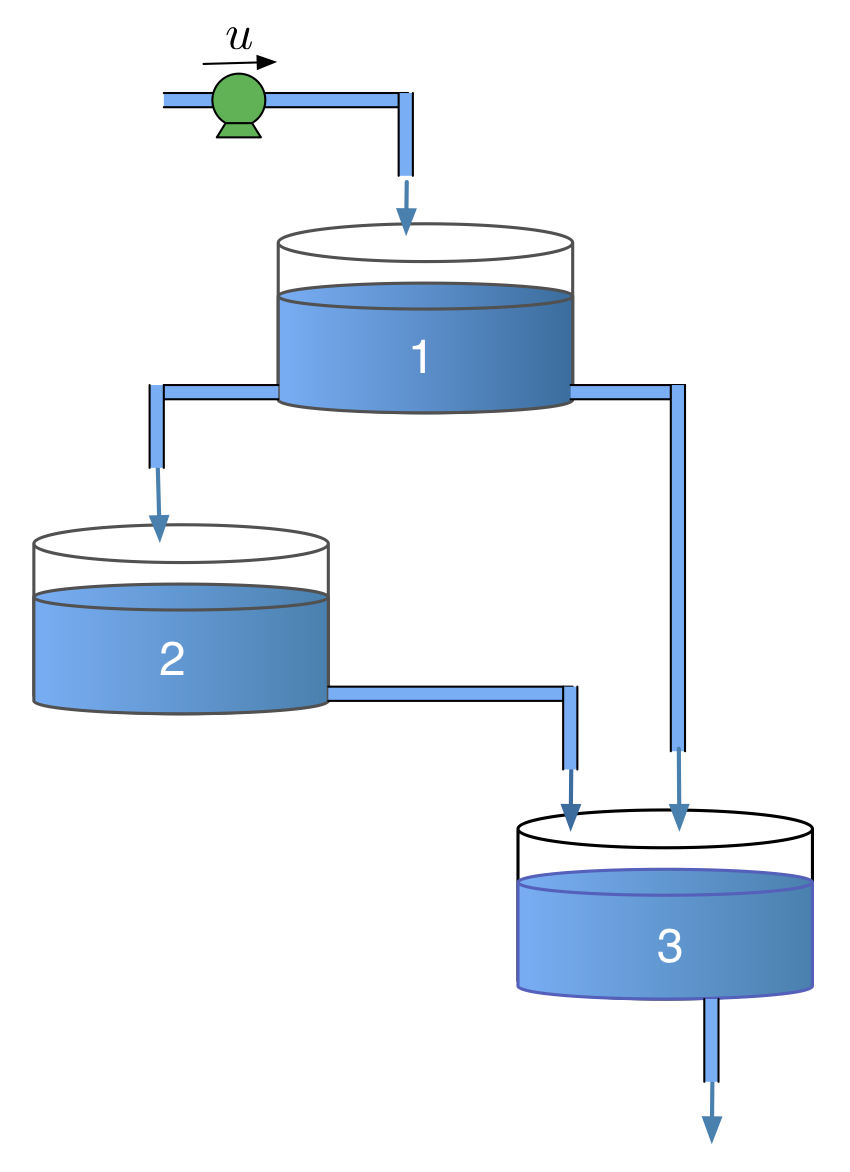
\includegraphics[width = .3\textwidth]{img/compartment.png}
\end{figure}
Defining $q(x,u)$ the vector of flows (in an arbitrary order), we get the matrix form:
\begin{equation}
    \dot x= Lq(x,u)
\end{equation}
where $L$ is the incidence matrix of the oriented graph whose coefficients all belong to $\{-1,0,1\}$. 
\begin{definition}
    A vector is nonnegative if each of its components is a nonnegative real number. The nonnegative orthant is the set of all nonnegative vectors of dimension $n$.
\end{definition}
\begin{definition}
    A dynamical system $\dot x=f(x,u)$ is nonnegative if, for every admissible input $u$, its state is confined in the nonnegative orthant when the initial state is nonnegative. 
\end{definition}
\begin{thm}
    A dynamical system $\dot x=f(x,u)$ is nonnegative if $f$ is continuously differentiable and if 
    \begin{equation}
        x\in \R^n_+, \: x_i=0\Longrightarrow \dot x_i\ge 0\qquad \forall i
    \end{equation}
\end{thm}
\begin{thm}
    Under the following conditions, a dynamical compartmental system $\dot x= Lq(x,u)$ is nonnegative.
    \begin{itemize}
        \item The functions $q_{ij}$ are nonnegative functions of their arguments on their domain of definition: $q_{ij}:\R^n_+\times \R^m\rightarrow \R_+: (x,u)\rightarrow q_{ij}(x,u)$.
        \item The functions $q_{ij}$ are continuous and differentiable functions of their arguments on their domain of definition.
        \item As there cannot be an outflow from an empty compoartment, the functions $q_{ij}$ verify the condition 
    \end{itemize}
    \begin{equation}
        x_i=0\Longrightarrow q_{ij}(x,u)=0\qquad \forall i
    \end{equation}
\end{thm}
\section{Reaction systems}
The number $n$ of species is finite and these species are denoted by $X_i$. A reaction is thus a set of $m$ reactions of the following form:
\begin{equation}
    \sum_{i=1}^n \gamma_{ij} X_i \rightarrow \sum_{i=1}^n\delta_{ij}X_i \qquad j = 1,\dots,m \qquad \gamma_{ij},\delta_{ij}\ge 0
\end{equation}
The coefficients $\gamma_{ij}$ and $\delta_{ij}$ are positives real numbers called stoichiometric coefficients. We create 3 matrices: 
\begin{itemize}
    \item $\Gamma = [\gamma_{ij}]$
    \item $\Delta = [\delta_{ij}]$
    \item $C = \Delta - \Gamma$
\end{itemize}
The rank $p$ of $C$ is called the reaction network rank, it is the number of independent reactions. 
\subsection{State-space model}
Let $x_i(t)$ denote the quantity of the species $X_i$ per unit of volume in the system at time $t$, and let $r_j:\R^n_+\rightarrow \R_+$ be the reaction rate associated to each reaction. It verifies 
\begin{itemize}
    \item $r_j(x)\ge 0$ $\forall j\: \forall x\in \R_+^n$
    \item $r_j(x)=0$ if $x_i=0$ for some $i\in I^{rj}$, $I^{rj}$ being the set of indices of all reactants involved in reaction $j$.
\end{itemize}
The equations of the system are thus
\begin{equation}
    \dot x_i = \sum_{j=1}^m (\delta_{ij}-\gamma_{ij})r_j(x(t))+\frac{1}{V}(Q_{0i}(t)-Q_{i0}(t))
\end{equation}
with $V$ the constant volume, $Q_{i0}(t)$ the flux going from the domain to the outside and $Q_{0i}(t)$ the flux going from the outside into the domain. In matrix form,
\begin{equation}
    \dot x= Cr(t)+q_{in}(x,u)-q_{out}(x,u)
\end{equation}
\subsection{Modelling of reaction kinetics}
\begin{equation}
    r_j(x) = k_j \prod_{i\in I^{rj}} x_i^{\nu_{ij}}
\end{equation}
where $k_j$ is the kinetic constant of the $j$th reaction, and $\nu_{ij}$ the partial order of the $i$th reactant in the $j$th reaction. Generally, $\nu_{ij}=\gamma_{ij}$. 
\subsection{Continuous Stirred Tank Reactors (CSTR)}
We study here a perfectly mixed chemical reactor of constant volume $V$\footnote{This is achieved by adjusting the in and out flowrates.}. We call $F_{in}$ the feed volumetric flowrate. The reactional equation of the system is, with $u\triangleq F_{in}/V$,
\begin{equation}
    \dot x = Cr(x)-ux+ux^{in}
\end{equation}
If the volume is not constant,
\begin{equation}
    \frac{d}{dt}(xV) = Cr(x)V-F_{out}x+F_{in}x^{in} 
\end{equation}
Balancing the volumes,
\begin{eqnarray}
    \dot V = F_{in}-F_{out}
\end{eqnarray}
and thus 
\begin{equation}
    \dot x = Cr(x) + \frac{u_1}{x_{n+1}}(x^{in}-x)\qquad \dot x_{n+1} = u_1-u_2 \qquad \begin{cases}
        u_1 = F_{in}\\
        u_2 = F_{out}\\
        x_{n+1} = V
    \end{cases}
\end{equation}
Note that in a closed system, $q_{in}=q_{out}=0$. And a system is conservative if there exists $\omega\in \R^n$ such that $C^T\omega=0$ and $\omega_i>0$ for all $i$.
\end{document}